\documentclass[germanthesis]{thesis-style}
% options:
% [germanthesis] - Thesis is written in German
% [plainunnumbered] - Don't print numbers on plain pages
% [earlydraft] - Settings for quick draft printouts
% [watermark] - Print current time/date at bottom of each page
% [phdthesis] - switch to PhD thesis style
% [twoside] - double sided
% [cutmargins] - text body fills complete page

% Extension to BibLaTex (useful for cites in footnotes)
%\usepackage[backend=bibtex, style=numeric-comp]{biblatex}
\bibliography{references}

% additional packages
\usepackage{color, colortbl} % colors (interface table)
%\usepackage{tabularx} % set table width
\usepackage{longtable}

\author{Daniel~Witsch}
\title{R-Paket für Kanalkodierung mit Turbokodes}
%\title{R~package for channel~coding with convolutional~codes}
\birthday{28. Dezember 1992}
\birthplace{Zams}
%\thesisstart{1. Januar 2009}
\thesistype{Bachelor's thesis}
\thesistypegerman{Bachelorarbeit}
\thesiscite{Bachelor's thesis}
\advisors{Dr.~Pascal~Schöttle}
\date{\today}

\begin{document}

% Titelseiten und Eidesstattliche Erklärung
\maketitle
% Deutsche Zusammenfassung
\abstract{% abstract.tex
Diese Bachelorarbeit beinhaltet die Implementierung von Faltungskodes in R. Faltungskodes sind ein häufig verwendeter Typ der Kanalkodierung um Nachrichten über einen Kanal, der die Nachrichten durch Rauschen verfälscht, zu senden. Dabei wird zur Information Redundanz hinzugefügt, sodass der Empfänger trotz fehlerhafter Übertragung die Originalnachricht dekodieren kann. Die implementierten Funktionen stehen in einem R-Paket zur Verfügung, welches Studierenden beim Untersuchen von Faltungskodes zu Lehrzwecken dient.}
% Literaturverzeichnis
\tableofcontents
\pagenumbering{arabic}

\chapter{Einleitung}
\label{cha:introduction}
Aufgrund der steigenden Anzahl von mobilen Anwendungsgeräten ist die Mobilkommunikation ein wichtiger Teilbereich der Nachrichtentechnik. Zur Datenübertragung werden elektromagnetische Funkwellen benutzt, die aufgrund der äußeren Umwelteinflüsse störanfälliger als kabelgebundene Übertragungskanäle sind. Deswegen benötigt es eine Technik, welche es dem Empfänger ermöglicht, die Fehler die aus den Störungen resultieren, beheben zu können. Dabei kommen die Verfahren der Kanalkodierung zum Einsatz. Diese ermöglichen es vor dem Absenden der Daten, zusätzliche Informationen zur Nachricht hinzuzufügen, um beim Empfang die entstandenen Fehler zu korrigieren.

Ein fortgeschrittenes Verfahren bei der Kanalkodierung sind die Turbo-Kodes. Diese kombinieren die bereits bekannten Kodierungen, wodurch ein Gesamtkode entsteht, dessen Leistungsfähigkeit nahe der maximalen theoretischen Übertragungsgrenze liegt. Aufgrund der langen Signallaufzeiten in der Mobil- und Satellitenkommunikation werden Turbo-Kodes eingesetzt, da bei einer fehlerhaften Übertragung ein erneutes Senden nicht praktikabel wäre. Deswegen kann aus den Informationen, die vor dem Versand hinzugefügt wurden, die Originalnachricht trotz Störungen wiederhergestellt werden. Schon seit den 1980er Jahren wird diese Art der Kodierung in Bereichen der Speichersysteme, wie CD oder DVD, eingesetzt. Für den heutigen Erfolg der Mobilfunkstandards LTE und UMTS ist dieses Verfahren ausschlaggebend, um die Übertragungsgeschwindigkeiten zu erreichen. Auch die bekannte ESA Raumsonde Rosetta, die seit August 2014 einen Kometen umkreist, benutzt diese Technik für die Kommunikation mit dem Kontrollzentrum auf der Erde.~\cite[S.~242~f.]{schoenfeld2012informations} 

Ziel dieser Arbeit war es, das Prinzip des Turbo-Kode-Verfahrens, mit der Programmiersprache R, in ein wiederverwendbares R-Paket zu implementieren. Für zukünftige Studierende sollte eine visuelle Darstellung geschaffen werden, die den prinzipiellen Ablauf der Kodierung und Dekodierung darstellt. Durch die praktische Anwendung und grafische Visualisierung soll das Verständnis von Turbo-Kodes erleichtert werden. Somit ist das R-Paket eine optimale Ergänzung zum theoretischen Unterricht an den Universitäten.

Die beiden weiteren Bachelorarbeiten \enquote{Kanalkodierung mit Blockkodes} von Benedikt Wimmer \cite{wimmer} und \enquote{Kanalkodierung mit Faltungskodes} von Martin Nocker \cite{nocker} vervollständigen das R-Paket, um die gesamte Funktionalität der Kanalkodierung zu integrieren. Dadurch erhalten die Studierenden ein kompaktes und einfach verwendbares R-Paket, welches alle wichtigen Bestandteile des Kanalkodierungsverfahren beinhaltet und eine hilfreiche visuelle Darstellung anbietet.   

Diese Bachelorarbeit startet in Kapitel~\ref{cha:basics} mit den Grundlagen der Kanalkodierung. Diese werden benötigt, um anschließende Verfahren besser verstehen zu können. Danach werden in Kapitel~\ref{cha:technologies} kurz die verwendeten Technologien und deren Vorteile erläutert. Die genaue Erklärung der Implementation des Paketes, wird in Kapitel~\ref{cha:implementation} veranschaulicht. Zur Verwendung der Funktionen finden sich in Kapitel~\ref{cha:interface} die Schnittstelle des Paketes. Um eine Hilfe bei dem Verständnis der Visualisierungen zu erhalten, werden in Kapitel~\ref{cha:visualization} alle wichtigen Darstellungen im Detail erklärt. Der Einsteig zur Verwendung des R-Paketes soll mit den Beispielen von Kapitel~\ref{cha:examples} erleichtert werden. Einige mögliche Erweiterungen werden zum Abschluss noch in Kapitel~\ref{cha:result} vorgebracht.

\chapter{Grundlagen und ähnliche Arbeiten}
\label{cha:basics}
In diesem Grundlagenkapitel werden alle wichtigen theoretischen Konzepte von Kanalkodierung und im speziellen zu Turbo-Kodes erklärt, um die Implementation in C- beziehungsweise R-Code, das in Kapitel \ref{cha:implementation} erläutert wird, zu verstehen. Die Notation und der Inhalt orientiert sich an dem Buch von Schönfeld \cite{schoenfeld2012informations}.

\section{Kanäle}
\label{sec:channels}
Um Nachrichten an den gewünschten Empfänger zu transportieren, können verschiedene Übertragungsmediums verwendet werden, wie zum Beispiel Kupferkabel oder Funkwellen. Jedes dieser hat spezielle Eigenschaften und Charakteristiken. Damit dieses mit einem Computerprogramm simuliert werden kann, muss ein Modell geschaffen werden, das einen solchen Übertragungskanal bestmöglich abbildet. Dieses Modell bildet alle Störungen und Dämpfungen ab, die während der Übertragung passieren können. Als ein gut geeignetes Modell stellte sich das Überlagern des Signals mit dem \emph{Additiv Weißes Gaußsches Rauschen} (AWGR) heraus \cite[81]{schoenfeld2012informations}. Dieses Rauschen wird folgenderweiße berechnet:

\begin{equation}
E_s = \frac{1}{L} \displaystyle\sum_{i=0}^{L-1} |x[i]|^2; \quad L = length(x)
\label{eq:power}
\end{equation}

In der Formel \ref{eq:power} wird zuerst die Länge der Nachricht ($x$ ist ein Vektor) berechnet, um im Anschluss über alle Bits zu iterieren und die Summe der Quadrate des Signals zu berechnen. Diese Summe wird dann noch durch die Länge dividiert, um die Leistung je Bit zu erhalten.

\begin{equation}
noise = \sqrt{\frac{E_s}{10^{dB/10}}} * randn(1,L)
\label{eq:noise}
\end{equation}

Das Signal/Rausch-Verhältnis muss zuerst vom Dezibel-Bereich in den Linearen umgerechnet, wie im Nenner der Wurzel in der Gleichung \ref{eq:noise} zu sehen ist.
Zur Berechnung des Rauschens werden $L$ Zufallszahlen zwischen 0 und 1 erzeugt und diese mit dem Wurzelergebnis multipliziert. 

\begin{equation}
y = x + noise
\label{eq:noisySignal}
\end{equation}

Danach wird einfach das Rauschen mit dem Originalsignal überlagert, um das verrauschte Signal zu erhalten. Dieses stellt nun den simulierten Übertragungskanal dar, die Stärke der Störung ist mittels der $dB$-Variable zu beeinflussen \cite{AWGN}.

\section{Kanalkodierung}
\label{sec:channelcoding}

\begin{figure}[t]
\centering
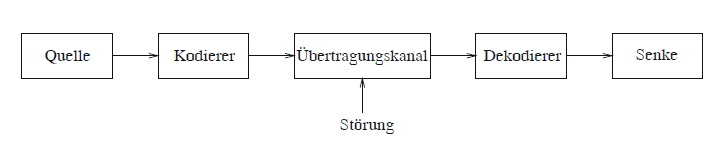
\includegraphics[width=\ScaleIfNeeded]{pictures/Channelmodel}
\caption{Modell der Nachrichtenübertragung, Quelle: \cite[10]{schoenfeld2012informations}}
\label{pic:channelmodel}
\end{figure}

In der Abbildung \ref{pic:channelmodel} ist ein generelles Modell der Nachrichtenübertragung dargestellt, das den Weg einer Nachricht zeigt. Nachdem der Sender (Quelle) die Nachricht durch den Quellenkodierer und Kanalkodierer geschickt hat, gelangt das Kanalwort auf den Übertragungskanal. Dort stören äußere Einflüsse das Signale und verändern es. Beim Empfänger wird versucht, die Nachricht wieder zu dekodieren und die Originalnachricht zu erhalten.

Das Ziel der Kanalkodierung dabei ist den Quellenkodewörtern Redundanz hinzuzufügen, um nach einer fehlerhaften Übertragung über das Übertragungsmedium, die Ausgangsnachricht wieder rekonstruieren zu können. Dabei können Fehler erkannt und im Bestem Fall sogar komplett korrigiert werden.

\subsection{Zweites SHANNONsches Kodierungstheorem}
\label{sec:shannonTheorem}
Auf dem Übertragungskanal wird die zu übertragende Information zu einer bestimmen Wahrscheinlichkeit verfälscht. Durch die Kanalkodierung können Fehler bis zu einem bestimmten Grad korrigiert werden, jedoch bleiben Fehler mit einer bestimmten Restwahrscheinlichkeit.

SHANNON\footnote{Wurde nach Claude Elwood Shannon und Ralph Hartley benannt.} hat mit seinem zweitem Theorem bewiesen, dass es theoretisch möglich ist eine Kanalkodierung zu finden, welche die Restfehlerwahrscheinlichkeit beliebig klein halten kann. Allerdings nur unter der Bedingung, dass der Sender weniger Kodewörter erzeugt, als der Kanaldekodierer beim Empfänger verarbeiten kann. Bereits 1948 erkannte SHANNON eine Grenze, die sogenannte SHANNON-Grenze, welche eine Grenze des Signal/Rausch-Verhältnisses, im Bezug auf die hinzugefügte Redundanz und der erreichbaren Restfehlerwahrscheinlichkeit darstellt. Somit wurde ein Ziel gesteckt mit einer geeigneten Kodierung dieser Grenze möglichst nahe zu kommen \cite[125 f.]{schoenfeld2012informations}.

Ein großer Schritt in Richtung dieser SHANNON-Grenze war im Jahre 1993 die Vorstellung der Turbo-Kodes. Mit denen war es erstmals möglich sehr nahe dieser Grenze zu kommen.

\subsection{Prinzipien der Fehlerkorrektur}
\label{sec:principlesMistakesCorrection}
Die hinzugefügte Redundanz kann auf ganz unterschiedliche Weisen erfolgen. Grundsätzlich gibt es 2 Möglichkeiten diese dem Quellenkodewort hinzuzufügen:

\begin{itemize}
\item Wiederholung der Nachricht
\item Rekonstruktion der Nachricht
\end{itemize}

Bei der ersten Möglichkeit fordert der Empfänger die Nachricht erneut an, wenn er bemerkt, dass die Nachricht nicht korrekt übertragen wurde. Den Fehler erkennen kann er durch Kontrollstellen in der Nachricht, zum Beispiel von Paritätsbits. Bei der zweiten Möglichkeit dient die hinzugefügte Redundanz nicht nur zur Erkennung der Fehler, sondern auch als Hilfe zur Rekonstruktion der Originalnachricht. Natürlicherweise muss die Redundanz größer sein, als bei der ersten Methode, die nur Fehler erkennt.

Es wird vorausgesetzt, dass die Wahrscheinlichkeit von Einzelfehlern größer ist, als das Auftreten von Bündelfehlern, also mehrere Fehler hintereinander. Jede Kodierung hat seine Grenze, deswegen kann auch der Beste Dekodierer nicht unendliche viele Fehler korrigieren. Zur Rekonstruktion des Kodewortes wird die \emph{Maximum-Likelihood-Methode} verwendet. Dabei wird das Kodewort gesucht, das einem existierendem, realistischen Wort am nähesten liegt. Dadurch liefert der Dekodierer immer ein Kodewort, das die geringste Distanz zum gesendeten Kodewort aufweist. Das bedeutet jedoch nicht, dass es unbedingt die richtige Nachricht sein muss. Der Berechnungsaufwand dieser Methode steigt allerdings mit der Länge der Nachricht enorm \cite[126-129]{schoenfeld2012informations}. 

\subsection{Verwendete Notation}
\label{sec:notation}
In den folgenden Kapiteln werden immer wieder Variablen verwendet, die aber nicht bei der konkreten Formel eingeführt werden. Deshalb wird in diesem Kapitel einmal die Variablen eingeführt und dann immer verwendet Bei diesen Definition werden immer Kodewörter mit dem Alphabet ${0,1}$ verwendet, da dieser Fall am meisten Bedeutung hat.

Nachrichten werden zuerst mit dem Quellenkodierer in eine möglichst redundanzfreie Form gebracht, um die verwendeten Bits möglichst gut auszunutzen. Diese Kodewörter werden als Quellenkodewörter bezeichnet und sind folgenderweise definiert:

\begin{t_def}
Ein Wort $a^* \in {0,1}^l$ wird als Quellenkodewort der Länge $l$ bezeichnet.
\end{t_def}

Im Anschluss wird Redundanz den Quellenkodewörtern durch den Kanalkodierer hinzugefügt, das resultierende Kodewort sieht folgenderweise aus:

\begin{t_def}
Ein Wort $a \in {0,1}^n$ wird als Kanalkodewort der Länge $n$ bezeichnet.
\end{t_def} 

Durch das hinzufügen von Redundanz ergeben sich $k = n - l$ redundante Stellen. Diese werden zur Fehlererkennung und Fehlerkorrektur bei der Dekodierung verwendet.

Zum Beispiel erzeugt ein Quellenkodierer Nachrichten der Länge $l=2$, $a^*_{1}=(00),a^*_{2}=(01),a^*_{3}=(10),a^*_{4}=(11)$. Danach fügt der Kanalkodierer eine redundante Stelle hinzu $k=1$, also haben die Nachrichten dann eine Länge von $n=3$. Sie könnten folgenderweise aussehen, $a_{1}=(001),a_{2}=(010),a_{3}=(100),a_{4}=(110)$.

\subsection{Kenngrößen von Kanalkodes}
\label{sec:channelParameters}
Für die Betrachtung von verschiedenen Kanalkodierungen ist es wichtig Unterscheidungsmerkmale zu finden. Diese werden in diesem Kapitel eingeführt. Dazu wird als erstes in Kapitel \ref{sec:hammingDistance} die Distanz zwischen zwei Kodewörtern erklärt, um im Anschluss in Kapitel \ref{sec:hammingWeight} das Gewicht eines Wortes berechnen zu können. Am Schluss in Kapitel \ref{sec:codeRate} wird noch der Begriff der Kode-Rate eingeführt.

\subsubsection{Hamming-Distanz}
\label{sec:hammingDistance}
Damit durch einzelne Fehler auf dem Übertragungskanal, nicht eine anderes existierende Nachricht produziert wird, sollen Kodewörter angestrebt werden, die sich möglichst weit unterscheiden. Eine wichtige Kenngröße dabei ist der Abstand zwischen zwei Kodewörtern:

\begin{t_def}
Anzahl der Stellen, in denen sich 2 Kodewörter $a_i$ und $a_j$ unterscheiden. Die Zahl nennt man die\emph{Hamming-Distanz} zwischen den beiden Wörtern.
\end{t_def} 
 
\begin{equation}
d(a_i,a_j) = \sum^{n}_{g=1} (u_{ig} \oplus u_{jg})
\label{eq:hammingDistance}
\end{equation}

Diese lässt sich bei Binärkodes mit der Formel \ref{eq:hammingDistance} berechnen, dabei wird einfach gezählt, wie viele Stellen sich unterscheiden. Interessant ist der kleinste Unterschied zwischen zwei Kodewörtern, die Zahl wird \emph{minimale Hamming-Distanz} $d_{min}$ genannt.

Ein Kode der alle Verfälschungen $\leq f_e$ erkennen kann, muss eine \emph{minimale Hamming-Distanz} von 

\begin{equation}
d_{min} = f_e + 1
\end{equation}

besitzen. Mit $f_e$ wird Grad der Fehlererkennung genannt. Die Anzahl der korrigierbaren Fehler $f_k$ lässt sich folgenderweise berechnen:

\begin{equation}
f_k = \frac{d_{min}-1}{2}
\end{equation}

Damit nun Fehler erkannt und korrigiert werden können, muss die \emph{minimale Hamming-Distanz} mindestens folgende Gleichung erfüllen \cite[132 f.]{schoenfeld2012informations}:

\begin{equation}
d_{min} = f_e + f_k + 1
\end{equation} 

\subsubsection{Hamming-Gewicht}
\label{sec:hammingWeight}

\subsubsection{Kode-Rate}
\label{sec:codeRate}

\section{Turbo-Kodes}
\label{sec:turboCodes}

\chapter{Verwendete Technologien}
\label{cha:technologies}
Die folgenden Kapitel sollen einen kleinen Überblick über die verwendete Technologien während der Bachelorarbeit liefern. Sie sollen auch Aufschluss darüber geben, wieso diese verwendet wurden und welche Vorteile sie besitzen. Zuerst wird in Kapitel \ref{sec:R} die Programmiersprache R und deren Entwicklungsumgebung RStudio erklärt, um im Anschluss in Kapitel \ref{sec:Rcpp} die Vorzüge vom Paket \emph{Rcpp} und die dabei verwendete Sprache C++ zu beschreiben. Am Ende wird in Kapitel \ref{sec:RMarkdown} über die Visualisierungsmöglichkeiten gesprochen, die dem Studenten helfen soll, die Abläufe des Turbo-Kode-Verfahrens besser zu verstehen. Dabei wird die Auszeichnungssprache \emph{RMarkdown} und die darin verwendeten Sprachkonstrukte näher erläutert.

\section{R, RStudio, Pakete}
\label{sec:R}
Die Programmiersprache R wurde 1992 von den beiden Statistikern  Ross Ihaka und Robert Gentleman an der Universität Auckland entwickelt. Dabei wurde die Sprache speziell für Anwendungsfälle im statistischen Bereich gebaut. Die Sprache baut auf den Vorgänger S auf und wird mit einen Kommandozeileninterpreter ausgeliefert. Dadurch dass der Quellcode nicht kompiliert, sondern nur interpretiert wird, ist er auf verschiedenen Plattformen ausführbar. Der kanadische Mitentwickler John M. Chambers beschreibt die Sprache folgenderweise:

\enquote{To understand computations in R, two slogans are helpful: Everything that exists is an object. Everything that happens is a function call.} \cite{chambers2014object}\\

Diese beiden Aussagen beschreiben, dass R nur aus Objekte und Funktionen besteht. Das bedeutet, dass jede Variable ein Objekt ist, das zur Laufzeit seine Struktur verändern kann. Somit ist R eine schwach, dynamisch typisierte Programmiersprache. Dadurch muss einer Variable kein Datentyp zugewiesen werden und die Typüberprüfung findet erst zur Laufzeit statt. Ein weiterer Grund R zu verwenden, ist die hervorragende Eigenschaft, große Datenmengen graphisch darzustellen. Dieses Problem lässt sich mit R hervorragend bewältigen.

Um den Funktionsumfang der Sprache zu erweitern, stehen zahlreiche Pakete auf den CRAN-Servern\footnote{The Comprehensive R Archive Network: \url{https://cran.r-project.org/}} zur Verfügung. Dort veröffentlicht die R-Community ihre entwickelten Pakete, um sie mit den restlichen Nutzern von R zu teilen. Damit ein selber entwickeltes Paket dort aufgenommen wird, muss es strenge Kriterien erfüllen, um die Qualität der Pakete zu sichern. Mittlerweile stehen über 8000 verschiedene Pakete (Stand: Mai 2016) auf den Servern zum Download bereit. Diese decken einen großen Anwendungsbereich ab und sind daher sehr hilfreich, um selbst R-Code zu entwickeln \cite{rmanual}.

Zwei sehr wichtige Pakete sind notwendig, um selbst R-Pakete zu entwickeln. Dazu zählt \emph{devtools}, das hilfreiche Funktionen für die Erstellung (Build) von Paketen zur Verfügung stellt. Damit werden viele Tätigkeiten automatisiert, die ansonsten vom Entwickler getätigt werden müssen. !!TODO ZITAT!!  Ein weiteres wichtiges Paket zur Unterstützung bei der Entwicklung eines Paketes ist \emph{roxygen}. Damit lässt sich ähnlich wie bei \emph{JavaDoc}, Kommentare in den Quellcode schreiben, die dann automatisch zu einer Paketdokumentation führen. Die \emph{roxygen}-Kommentare starten mit #'. Die wichtigsten Annotation sind für die Parameter (@param) und für den Rückgabewert (@return). Es können auch Beispiele (@examples) eingebunden werden, die dann automatisch bei der Erstellung getestet werden, ob sie richtig funktionieren. Wahrscheinlich die wichtigste Annotation bei der Entwicklung ist die Veröffentlichung einer Funktion im Paket (@export), dadurch wird sichergestellt, dass der Benutzer Zugriff zu dieser Funktion hat.

\begin{figure}[t]
\centering
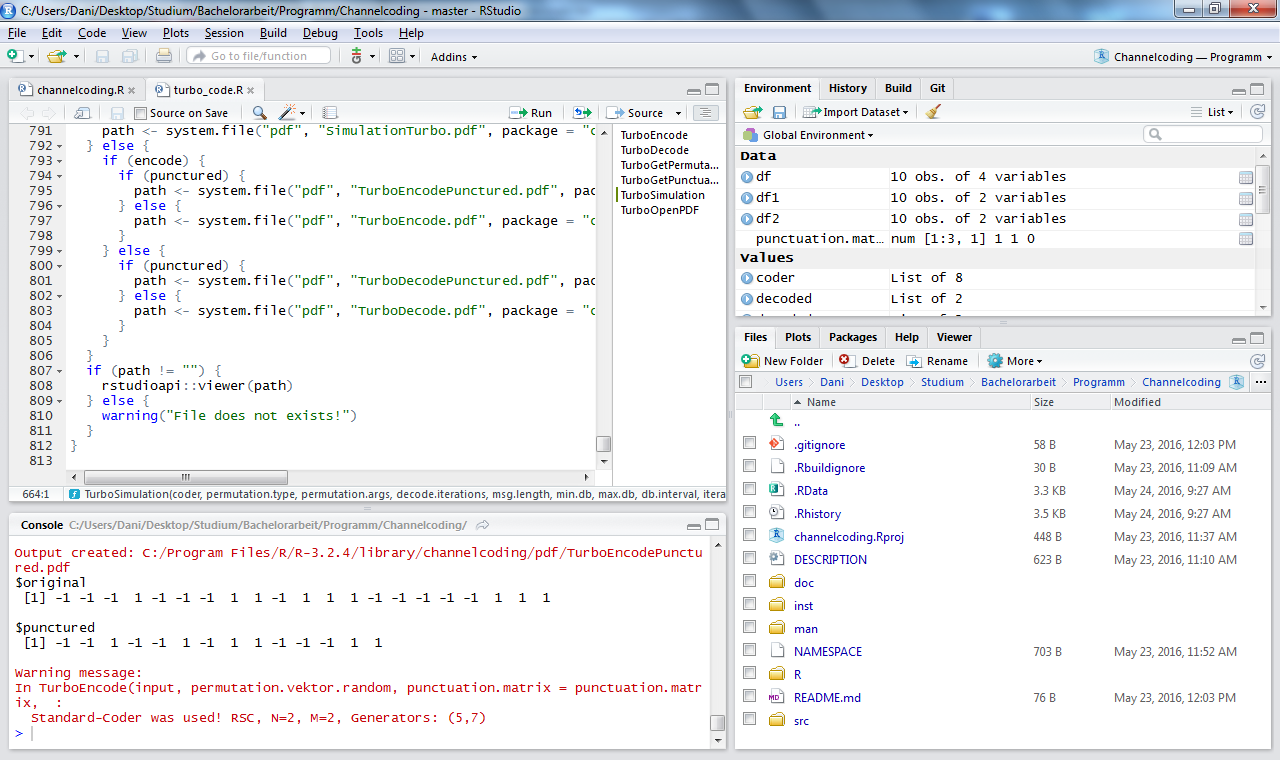
\includegraphics[width=\ScaleIfNeeded]{pictures/RStudio}
\caption{RStudio Standartansicht}
\label{pic:RStudio}
\end{figure}

Die weitverbreiteste Entwicklungsumgebung für die Programmiersprache R ist das RStudio, das in der Abbildung \ref{pic:RStudio} zu sehen ist. Diese Umgebung wurde speziell für den Softwareentwurf mittels R entwickelt und stellt alle wichtigen Funktionen zu Verfügung. Damit ist es besonders einfach selber R-Pakete zu entwickeln, oder andere Programmiersprachen mittels speziellen Schnittstellen mit R zu verbinden. Zur Visualisierung von den Berechnungsergebnissen sind bereits einige Vorlagen in die Entwicklungsumgebung integriert. Zum Beispiel ist es sehr einfach HTML Seiten, PDF Dokumente oder auch interaktive Oberflächen mittels \emph{Shiny} zu erstellen. Um dynamische Dokumente zu erstellen kann auch \emph{RMarkdown} verwendet werden, das wird im Kapitel \ref{sec:RMarkdown} näher erklärt.

\section{C++, Rcpp}
\label{sec:Rcpp}
In manchen Situationen ist R nicht schnell genug für die spezielle Anwendung, deswegen kann man auf C oder C++ zurückgreifen. Vorallem die Geschwindigkeit bei Schleifen ist aufgrund der schwachen Typisierung in R relativ schlecht. Darum kann man bei einer intensiven Nutzung von Schleifen auf C oder C++ zurückgreifen und mit einer speziellen Schnittstelle diesen Code von R aufrufen.

Grundsätzlich gibt es drei Möglichkeiten C/C++-Code von R aufzurufen:
\begin{itemize}
	\item \emph{.C} native Schnittstelle
	\item \emph{.Call} Schnittstelle
	\item \emph{Rcpp} Paket
\end{itemize}

Bei der ersten Möglichkeit handelt es sich um die einfachste Möglichkeit C-Code in R auszuführen. Dabei hat der C-Code keinerlei Informationen über die R-Datentypen, sondern erhält als Argumente nur Zeiger auf bestimmte Speicherstellen. Als Rückgabe einer Funktion müssen wieder Zeiger verwendet werden, für die bereits im R-Code Speicherplatz reserviert werden musste.

Die \emph{.Call}-Schnittstelle ist eine Erweiterung der \emph{.C}-Schnittstelle. Sie ist wesentlich schwieriger zu verwenden, bietet allerdings einige hilfreiche Features. Zum Beispiel ist es möglich R-Datentypen direkt zu verwenden und auch die Rückgabe eines Wertes an R, kann einfach mit der normalen Rückgabe in einer C-Funktion erfolgen \cite{wickham2015r}.

Die empfohlene Variante mittlerweile ist die Verwendung des Paketes \emph{Rcpp}, weil dadurch der C++-Code übersichtlich bleibt und der Benutzer viele hilfreiche R-Datentypen zur Verfügung hat. (Vektoren, Matrizen, Listen, ...) Noch dazu gibt es einige Funktionen die in C++ gleich verwendet werden können wie in R, zum Beispiel ist es möglich der Wurzelfunktion einen ganzen Vektor als Parameter mitzugeben und erhält dann einen Vektor retour, von dem jeder einzelne Wert die Wurzel gezogen wurde. In der STL-Bibliothek sind viele weitere Datenstrukturen und Algorithmen die im C++-Code verwendet werden können und somit das Leben des Programmierers erleichtern können. Durch die gute Integration von \emph{Rcpp} in die Entwicklungsumgebung RStudio ist es sehr einfach bei der Entwicklung von einem Paket C++-Code zu verwenden. Beim Erzeugen des Paketes kompiliert RStudio automatisch alle C++-Dateien und erstellt automatisch Wrapper-Funktionen, die den Zugriff auf die Funktionen erleichtern. Die genaue Verwendung von diesem \emph{Rcpp}-Paket ist im Buch von Hadley Wickham nachzulesen \cite{wickham2015advanced}. 

\section{RMarkdown, \LaTeX, Ti\textit{k}Z}
\label{sec:RMarkdown}
Mittels dem Paket \emph{RMarkdown} lassen sich sehr einfach dynamische Dokumente im RStudio erzeugen. Dabei wird grundsätzlich die Auszeichnungssprache Markdown verwendet, jedoch lassen sich einfach R-, \LaTeX - und HTML-Code in die \emph{RMarkdown}-Datei (.rmd Dateiendung) integrieren. Dadurch hat man ein flexibles Werkzeug, um personalisierte Dokumente zu erstellen. Das Ausgabeformat kann einfach in den Kopfzeilen der Datei bestimmt werden. Dabei sind folgende Formate möglich: HTML, PDF, Word, RTF, ODT oder einfaches Markdown. Noch dazu ist es sehr einfach eine Präsentation zu erstellen, da mit einfachen Befehlen im Quellcode neue Folien erzeugt oder Auflistungen erzeugt werden können.

\begin{figure}[t]
\centering
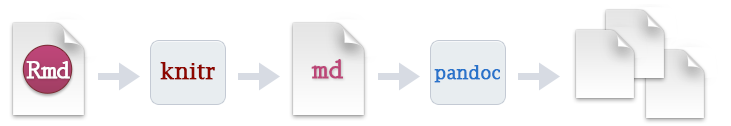
\includegraphics[width=\ScaleIfNeeded]{pictures/RMarkdown}
\caption{RMarkdown Überblick, Quelle: \cite{rmarkdown}}
\label{pic:RMarkdown}
\end{figure}

Der Arbeitsablauf ist ganz einfach, wie in der Abbildung \ref{pic:RMarkdown} zu sehen ist. Nach der Erstellung der RMD-Datei wird mit dem Paket \emph{knitr} der R-Code in der Datei ausgeführt und die Ergebnisse in die resultierende Datei, normale Markdown-Datei (.md Dateiendung), eingefügt. Im Anschluss wird mittels dem Programm \emph{pandoc}, das bereits in das RStudio integriert ist, die Datei in das Ausgabeformat gebracht. Somit lässt sich mit wenigen Schritten, dynamisch erzeugte Daten mittels R-Code, in eine schön formatierte Präsentation im PDF-Format unterbringen. Diesen gesamten Ablauf kapselt das \emph{RMarkdown}-Paket in einen einzigen Funktionsaufruf. (\emph{render}-Funktion) Dadurch wird für den Benutzer der Prozess wesentlich vereinfacht und er kann sich auf das Grundsätzliche, nämlich der Programmierung bzw. der Erstellung der RMD-Datei konzentrieren \cite{rmarkdown}.

Für dynamische Grafiken wurde die Sprache Ti\textit{k}Z verwendet, die in \LaTeX integriert wird. Mit dieser Kombination lassen sich schöne Grafiken dynamisch aufbauen mit relativ kompakten Code. Die Klasse Beamer in \LaTeX ermöglicht es Präsentationen zu erzeugen und somit Inhalte mittels verschiedenen Einblendungen darzustellen. Mit dieser Fähigkeit lassen sich auch verschiedene Bereiche in einer Ti\textit{k}Z-Zeichnung hintereinander einblenden, dadurch erhält der Benutzer einen besseren Überblick, wie die Grafik entsteht und kann daraus besser ableiten, wie der Vorgang abgelaufen ist. Diese Tatsache ist vor allem wichtig, wenn sich zukünftige Studenten die Visualisierungsfolien von der Kodierung und Dekodierung anschauen, da dort der genaue Ablauf mit Hilfe von verschiedenen Grafiken erklärt ist. Durch den langsamen Aufbau der Grafiken soll es dem Studenten erleichtern, das Prinzip des Turbo-Kode-Verfahrens zu verstehen. Mit dieser visuellen Unterstützung sollen die in der Vorlesung theoretisch erklärten Abläufe vertieft und praktisch mit den R-Funktionen umgesetzt werden.  

\startlist[Funktionen]{lot}
\chapter{R Paket Schnittstelle}
\label{cha:interface}
\definecolor{lightblue}{RGB}{150,180,255}
Dieses Kapitel soll als zusätzliche Hilfe (Nachschlagewerk) bei der Verwendung der R-Funktionen dienen, da hier die genauen Schnittstellen der Funktionen erklärt werden. Nachdem das Paket installiert ist, steht die Hilfe auch im RStudio zur Verfügung. Diese ist allerdings auf Englisch und nicht so umfangreich. Falls nach diesem Kapitel die Verwendung noch nicht komplett klar ist, kann man sich auch die Beispiele in Kapitel~\ref{cha:examples} anschauen. Für eine genaue Erklärung der Funktionen kann in Kapitel~\ref{cha:implementation} die genaue Implementierung nachgelesen werden und daraus auf die weitere Verwendung geschlossen werden.

In Kapitel~\ref{sec:interface_turboFunctions} sind alle Funktionen gelistet, die für das Kodieren und Dekodieren notwendig sind. Ein paar Hilfsfunktionen sind in Kapitel~\ref{sec:interface_helperFunctions} nachzuschlagen und die allgemeinen Funktionen, die für alle drei Verfahren notwendig sind, können im Kapitel~\ref{sec:interface_channelFunctions} nachgelesen werden. 
\newpage

\section{Turbo-Kode Funktionen}
\label{sec:interface_turboFunctions}

\subsection{Kodieren}
\label{sec:interface_encode}
\begin{longtable}{|p{\textwidth}|}
\hline
\rowcolor{lightblue}TurboEncode\\
\hline
\\
\texttt{TurboEncode(message, permutation.vector, coder.info, parity.index, punctuation.matrix, visualize)}\\
\\
Kodiert eine Nachricht mittels dem Turbo-Kode-Verfahren. Dabei wird die Nachricht in zwei systematische Kodierer geschickt und am Ausgang wird das Ergebnis der beiden Kodierer mit der Originalnachricht zusammengesetzt. Falls eine Punktierungsmatrix mitgegeben wird, erfolgt am Ende die Punktierung und somit die Erhöhung der Koderate.\\
\\
\textbf{Argumente:}\\
\texttt{message} - Nachricht die kodiert wird. (0er und 1er)\\
\texttt{permutation.vector} - Permutationsvektor der für den Interleaver verwendet wird. Standard: \texttt{PRIMITIVE (root=0)}\\
\texttt{coder.info} - Faltungskodierer der mit den Funktionen \texttt{ConvGenerateEncoder, ConvGenerateRscEncoder} erzeugt werden kann. Muss ein systematischer Kodierer sein, also ein RSC oder Ausgang 1 muss durchgeschalten sein. Standard: \texttt{ConvGenerateRscEncoder(2,2,c(5,7))}\\
\texttt{parity.index} - Gibt an welcher Ausgang vom mitgegebenen Kodierer verwendet wird. Standard: letzter Ausgang\\
\texttt{punctuation.matrix} - Die Matrix wird am Ende des Kodiervorgangs zur Punktierung verwendet. Standard: keine Punktierung\\
\texttt{visualize} - Wenn \texttt{TRUE} wird PDF-Bericht erstellt. Standard: \texttt{FALSE}\\
\\
\textbf{Rückgabewert:}\\
Die kodierte Nachricht mit den Signalwerten -1 und 1, welche die Bits 1 und 0 darstellen. Falls punktiert wurde, wird eine Liste mit dem Originalkode und dem punktierten Kode zurückgegeben.\\
\\
\hline
\caption[TurboEncode]{TurboEncode - Funktionserklärung}
\end{longtable}

\subsection{Dekodieren}
\label{sec:interface_decode}
\begin{longtable}{|p{\textwidth}|}
\hline
\rowcolor{lightblue}TurboDecode\\
\hline
\\
\texttt{TurboDecode(code, permutation.vector, iterations, coder.info, parity.index, punctuation.matrix, visualize)}\\
\\
Dekodiert eine Nachricht mittels dem Turbo-Kode-Verfahren. Dabei werden zuerst die Punktierungsbits wieder eingefügt, falls Punktierung verwendet wurde. Danach erfolgt die Dekodierung, wobei die Ergebnisse der Dekodierer als Eingang des Nächsten verwendet werden. Dieser Vorgang wird mehrmals iterativ ausgeführt, je nach Anzahl der gewählten Iterationen.\\
\\
\textbf{Argumente:}\\
\texttt{code} - Nachricht die dekodiert wird. Der genaue Signalpegel wird verwendet.\\
\texttt{permutation.vector} - Permutationsvektor der für den Interleaver verwendet wird. Standard: \texttt{PRIMITIVE (root=0)}\\
\texttt{iterations} - Anzahl der Dekodierungsiterationen. Standard: 1\\
\texttt{coder.info} - Faltungskodierer der bei der Kodierung bereits verwendet wurde. Standard: \texttt{ConvGenerateRscEncoder(2,2,c(5,7))}\\
\texttt{parity.index} - Gibt an welcher Ausgang vom mitgegebenen Kodierer verwendet wird. Standard: letzter Ausgang\\
\texttt{punctuation.matrix} - Die mitgegebene Punktierungsmatrix wird am Anfang des Dekodiervorgangs,  für das Einfügen der jeweiligen Bits verwendet. Standard: keine Punktierung\\
\texttt{visualize} - Wenn \texttt{TRUE} wird PDF-Bericht erstellt. Standard: \texttt{FALSE}\\
\\
\textbf{Rückgabewert:}\\
Liste welche die dekodierte Nachricht und die genau berechneten Soft-Werte enthält.\\
\\
\hline
\caption[TurboDecode]{TurboDecode - Funktionserklärung}
\end{longtable}
\newpage

\subsection{Simulation von Turbo-Kodes}
\label{sec:interface_simulation}
\begin{longtable}{|p{\textwidth}|}
\hline
\rowcolor{lightblue}TurboSimulation\\
\hline
\\
\texttt{TurboSimulation(coder, permutation.type, permutation.args, decode.iterations, msg.length, min.db, max.db, db.interval, iterations.per.db, punctuation.matrix, visualize)}\\
\\
Automatische Simulation eines Kodierungs- und Dekodierungsverfahrens von Turbo-Kodes. Nach dem Kodieren wird der resultierende Kode verrauscht und im Anschluss dekodiert. Für das jeweilige Signal/Rausch-Verhältnis wird dieses Verfahren mehrmals (\texttt{iterations.per.db}) wiederholt und am Ende ein Durchschnitt der Bitfehlerrate berechnet.\\
\\
\textbf{Argumente:}\\
\texttt{coder} - Kodierer der für Kodierung und Dekodierung verwendet wird. Kann mittels den Funktionen \texttt{ConvGenerateEncoder, ConvGenerateRscEncoder} erzeugt werden. Standard: \texttt{ConvGenerateRscEncoder(2,2,c(5,7))}\\
\texttt{permutation.type} - Typ des Permutationsvektors. Standard: \texttt{PRIMITIVE}\\
\texttt{permutation.args} - Argumente für die Erzeugung des Permutationsvektors. Standard: \texttt{list(root=0)}\\
\texttt{decode.iterations} - Anzahl von Iterationen bei der Dekodierung. Standard: 5\\
\texttt{msg.length} - Länge der Nachricht. Standard: 100\\
\texttt{min.db} - Untergrenze des Signal/Rausch-Verhältnisses. Standard: 0.1\\
\texttt{max.db} - Obergrenze des Signal/Rausch-Verhältnisses. Standard: 2.0\\
\texttt{db.interval} - Schrittweite pro Erhöhung des Signal/Rausch-Verhältnisses. Standard: 0.1\\
\texttt{iterations.per.db} - Iterationen pro Signal/Rausch-Verhältnis zur Durchschnittsbildung. Standard: 100\\
\texttt{punctuation.matrix} - Verwendete Punktierungsmatrix. Standard: wird nicht punktiert\\
\texttt{visualize} - Wenn \texttt{TRUE} wird PDF-Bericht erstellt. Standard: \texttt{FALSE}\\
\\
\textbf{Rückgabewert:}\\
Dataframe das für jedes Signal/Rausch-Verhältnis eine Bitfehlerrate beinhaltet.\\
\\
\hline
\caption[TurboSimulation]{TurboSimulation - Funktionserklärung}
\end{longtable}

\section{Hilfsfunktionen}
\label{sec:interface_helperFunctions}

\subsection{Permutationsvektor erzeugen}
\label{sec:interface_permutation}
\begin{longtable}{|p{\textwidth}|}
\hline
\rowcolor{lightblue}TurboGetPermutation\\
\hline
\\
\texttt{TurboGetPermutation(message.length, coder.info, type, args, visualize)}\\
\\
Erzeugt einen Permutationsvektor für die Interleaver beim Turbo-Kode-Verfahren. Dabei können verschiedene Typen von Permutationen ausgewählt werden (RANDOM, PRIMITIVE, CYCLIC, BLOCK, HELICAL, DIAGONAL). Die genauere Erklärung des jeweiligen Typs findet sich im Kapitel \ref{cha:implementation}. Den jeweiligen Typen müssen spezielle Argumente in einer Liste mitgegebenen werden:
\begin{itemize}
\item RANDOM: Benötigt keine Argumente, wird komplett zufällig erstellt.
\item PRIMITVE: Erzeugt einen Vektor (1,2,3...) und schiebt diesen um den \emph{root}-Wert.
\item CYCLIC: Benötigt die Argumente \emph{cols} und \emph{rows} für die Erzeugung der Matrix und \emph{distance} um den Permutationsvektor zu erzeugen.
\item BLOCK: Benötigt die Argumente \emph{cols} und \emph{rows} für die Erzeugung der Matrix. Matrix wird von links nach rechts befüllt und von oben nach unten ausgelesen.
\item HELICAL: Benötigt die Argumente \emph{cols} und \emph{rows} für die Erzeugung der Matrix. Matrix wird von links nach rechts befüllt und von links oben nach rechts unten ausgelesen.
\item DIAGONAL: Benötigt die Argumente \emph{cols} und \emph{rows} für die Erzeugung der Matrix. Matrix wird von links nach rechts befüllt und dann diagonal ausgelesen.
\end{itemize} \\
\\
\textbf{Argumente:}\\
\texttt{message.length} - Länge der Nachricht die kodiert werden möchte.\\
\texttt{coder.info} - Faltungskodierer der mit den Funktionen \emph{ConvGenerateEncoder, ConvGenerateRscEncoder} erzeugt werden kann. Standard: \emph{ConvGenerateRscEncoder(2,2,c(5,7))}\\
\texttt{type} - Typ des erzeugten Permutationsvektors. Standard: RANDOM\\
\texttt{args} - Argumente für den jeweiligen Typ in einer Liste. Standard: NULL\\
\texttt{visualize} - Wenn TRUE wird die Permutationsmatrix dargestellt. Standard: FALSE\\
\\
\textbf{Rückgabewert:}\\
Permutationsvektor mit der richtigen Länge für die mitgegebene Nachricht und Kodierer.\\
\\
\hline
\caption{TurboGetPermutation - Funktionserklärung}
\end{longtable}

\subsection{Punktierungsmatrix erzeugen}
\label{sec:interface_punctuation}
\begin{longtable}{|p{\textwidth}|}
\hline
\rowcolor{lightblue}TurboGetPunctuationMatrix\\
\hline
\\
\texttt{TurboGetPunctuationMatrix(punctuation.vector, visualize)}\\
\\
Erzeugt eine Punktierungsmatrix von einem mitgegebenen Vektor für das Turbo-Kode-Verfahren (drei Zeilen). Es dürfen keine Null-Spalten entstehen!\\
\\
\textbf{Argumente:}\\
\texttt{punctuation.vector} - Vektor der in eine Punktierumatrix transformiert wird. Eine 1 behaltet das Bit, eine 0 verwirft das Bit.\\
\texttt{visualize} - Wenn \texttt{TRUE} wird Punktierungsmatrix dargestellt. Standard: \texttt{FALSE}\\
\\
\textbf{Rückgabewert:}\\
Punktierungsmatrix die für das Turbo-Kode-Verfahren geeignet ist.\\
\\
\hline
\caption[TurboGetPunctuationMatrix]{TurboGetPunctuationMatrix - Funktionserklärung}
\end{longtable}
\newpage

\subsection{Öffnen der erzeugten Visualisierungen}
\label{sec:interface_openPDF}
\begin{longtable}{|p{\textwidth}|}
\hline
\rowcolor{lightblue}TurboOpenPDF\\
\hline
\\
\texttt{TurboOpenPDF(encode, punctured, simulation)}\\
\\
Öffnet die mit \emph{TurboEncode, TurboDecode, TurboSimulation} bereits erzeugten PDF-Berichte. Die Dateien liegen im Paket-Ordner im Installationsverzeichnis von R.\\
\\
\textbf{Argumente:}\\
\texttt{encode} - Wenn TRUE werden PDFs vom Kodierungs-, bei FALSE vom Dekodierungsverfahren geöffnet. Standard: TRUE\\
\texttt{punctured} - Wenn TRUE werden PDFs mit Punktierungsverfahren geöffnet. Standard: FALSE\\
\texttt{simulation} - Wenn TRUE öffnet sich der Bericht der Simulation. Standard: FALSE\\
\\
\hline
\caption{TurboOpenPDF - Funktionserklärung}
\end{longtable}
\newpage

\section{Kanalkodierungsfunktionen im Paket}
\label{sec:interface_channelFunctions}

\subsection{Rauschen hinzufügen}
\label{sec:interface_applyNoise}
\begin{longtable}{|p{\textwidth}|}
\hline
\rowcolor{lightblue}
ApplyNoise\\
\hline
\\
\texttt{ApplyNoise(msg, SNR.db, binary)}\\
\\
Verrauscht ein Signal basierend auf das AWGN (additive white gaussian noise) Modell. Das ist das Standardmodell für die Simulation eines Übertragungskanals.\\
\\
\textbf{Argumente:}\\
\texttt{msg} - Nachricht die verrauscht wird.\\
\texttt{SNR.db} - Signal/Rausch-Verhältnis des Übertragungskanals. Standard: 3.0\\
\texttt{binary} - Blockkode-Parameter. Nicht zu verwenden! Standard: FALSE\\
\\
\textbf{Rückgabewert:}\\
Verrauschtes Signal.\\
\\
\hline
\caption{ApplyNoise - Funktionserklärung}
\label{func:applynoise}
\end{longtable}

\subsection{Simulation von Block-, Faltungs- und Turbo-Kodes}
\label{sec:interface_channelcodingSimulation}
% ChannelcodingSimulation.tex
\begin{longtable}{|p{\textwidth}|}
\hline
\rowcolor{lightblue}ChannelcodingSimulation\\
\hline
\\
\texttt{ChannelcodingSimulation(msg.length, min.db, max.db, db.interval, iterations.per.db, turbo.decode.iterations, visualize)}\\
\\
Simulation of channelcoding techniques (blockcodes, convolutional codes and turbo codes) and comparison of their bit-error-rates.\\
\\
\textbf{Arguments:}\\
\texttt{msg.length} - Message length of the randomly created messages to be encoded. Default: 100\\
\texttt{min.db} - Minimum SNR to be tested. Default: 0.1\\
\texttt{max.db} - Maximum SNR to be tested. Default: 2.0\\
\texttt{db.interval} - Step between two SNRs tested. Default: 0.1\\
\texttt{iterations.per.db} - Number of encode and decode processes per SNR. Default: 100\\
\texttt{turbo.decode.iterations} - Number of decoding iterations inside the turbo decoder. Default: 5\\
\texttt{visualize} - If true a PDF report is generated. Default: FALSE\\
\\
\textbf{Returns:}\\
Distorted message containing noise.\\
\\
\hline
\end{longtable}

\subsection{Darstellung verschiedener Simulationen}
\label{sec:interface_plotSimulationData}
% PlotSimulationData.tex
\begin{longtable}{|p{\textwidth}|}
\hline
\rowcolor{lightblue}PlotSimulationData\\
\hline
\\
\texttt{PlotSimulationData(\dots)}\\
\\
Stellt mehrere mitgegebene Dataframes in einem Diagramm dar. Damit kann man verschiedene Kanalkodierungsverfahren miteinander vergleichen.\\
\\
\textbf{Argumente:}\\
\texttt{\dots} - Dataframes die mit den Simulationsfunktionen erzeugt wurden.\\	
\\
\hline
\caption[PlotSimulationData]{PlotSimulationData - Funktionserklärung}
\end{longtable}
\stoplist[Funktionen]{lot}

\chapter{Implementierung}
\label{cha:implementation}
Bei den Implementierungen der Funktionen wird am Anfang immer überprüft, ob die Parameter richtig gesetzt wurden und alle mitgegebene Daten korrekt sind. Diese Überprüfungen werden bei der Erklärung nur dann ausgeführt, wenn sie speziell für diese Funktion von Bedeutung sind. 

Wenn nicht alle Parameter verwendet wurden, werden immer bestimmte Standardwerte gesetzt. Diese können in Kapitel~\ref{cha:interface} nachgelesen werden, die Erzeugung dieser wird hier jedoch nicht vorgestellt.

Sämtliche Hilfsfunktionen oder selbsterklärende Implementationen können im Code nachgelesen werden. Zur Erstellung aller Grafiken wird das Pakete \emph{ggplot2} verwendet. Die genauen Erklärungen zu diesen Funktionen findet sich im Buch zum Pakete~\cite{ggplot2}.

In Kapitel~\ref{sec:implementation_package} werden alle grundlegende Informationen zur Erstellung eines Paketes geliefert. Danach erfolgt die genaue Erklärung der Implementierung von der Erzeugung des Permutationsvektor in Kapitel~\ref{sec:implementation_permutation} und der Punktierungsmatrix in Kapitel~\ref{sec:implementation_puncturing}. Im Anschluss folgt die Kodierung~\ref{sec:implementation_encode} und Dekodierung~\ref{sec:implementation_decode}, um danach noch das Erzeugen des Rauschens in Kapitel~\ref{sec:implementation_applyNoise} zu erläutern. Zum Abschluss wird noch die Implementierung der Simulationen in Kapitel~\ref{sec:implementation_simulation} vorgestellt, als letztes erfolgt ein kleiner Einblick in die Erzeugung der Visualisierungen~\ref{sec:implementation_visualization}.

\section{Erstellung eines Paketes in RStudio}
\label{sec:implementation_package}
Pakete sind die Basis bei der Erzeugung wiederverwendbaren R-Codes. Dabei beinhalten Pakete Funktionen, Dokumentation zu den Funktionen und Beispieldaten. Die Erstellung eines eigenen Paketes ist mit der Entwicklungsumgebung RStudio sehr einfach und benötigt nicht viel Einarbeitungszeit.

Pakete werden mittels CRAN-Servern\footnote{The Comprehensive R Archive Network: \url{https://cran.r-project.org/}} geteilt, somit gibt es eine Quelle, von denen alle Entwickler die Pakete beziehen. Zur Installation eines Paketes kann RStudio oder der erste Befehl im Listing~\ref{lst:install} verwendet werden. Zur Entwicklung eines Paketes sind einige Hilfspakete nützlich, die bereits in Kapitel~\ref{cha:technologies} eingeführt wurden. 

\begin{lstlisting}[caption=Installation eines Paketes und dessen Abhängigkeiten, label={lst:install}, float=!th]
install.package()
install_deps(dependencies = TRUE)
\end{lstlisting}

Sollte C/C++-Code verwendet werden, müssen natürlicherweise ein Compiler und weitere Tools (in Windows RTools) am Entwicklungsrechner installiert sein. Genaue Informationen finden sich im Buch von Hadley Wickham~\cite[S.~18~ff.]{wickham2015r}.

Ein Paket wird mittels Wizard von RStudio (\emph{File$\rightarrow$New Project$\rightarrow$New Directory$\rightarrow$R Package}) erstellt. Dabei wird ein Ordner für das Paket erstellt, welcher eine DESCRIPTION- und eine NAMESPACE-Datei beinhaltet. Zusätzlich wird noch ein R-Ordner erstellt, der sämtliche R-Skripte (Funktionen) enthalten wird. Sollte C/C++-Code verwendet werden, muss dieser in den src-Ordner abgelegt werden. Alle Dateien im inst-Ordner werden automatisch bei der Installation kopiert, sind also vom R-Code aus erreichbar \cite[S.~196~ff.]{wickham2015r}. Noch dazu sind viele weitere Ordner, die allerdings nicht gebraucht wurden, in der Paketstruktur möglich.~\cite[S.~28~ff.]{wickham2015r}

In der DESCRIPTION-Datei werden alle wichtigen Informationen für das Paket gespeichert. Dies sind Entwicklerdaten, eine Kurzbeschreibung, Lizenzierung und eine Versionierung. Dort können auch benötigte Pakete angegeben werden, die bei der Installation vom CRAN-Server automatisch installiert werden. Bei einer lokalen Installation müssen diese Pakete selbständig nachinstalliert werden. Dies lässt sich einfach mit dem zweiten Befehl des Listings~\ref{lst:install} erledigen. Diese Funktion ist im Paket \emph{devtools} enthalten.~\cite[67-82]{wickham2015r}

Der Code wird mittels \emph{roxygen}-Kommentare dokumentiert. Dabei werden Kommentare in den Code eingefügt, die beim Erstellen des Paketes automatisch in eine Paket-Dokumentation umgewandelt werden. Die wichtigsten Annotationen wurden bereits in Kapitel~\ref{sec:R} vorgestellt.~\cite[83-110]{wickham2015r}

Die NAMESPACE-Datei verwaltet das Exportieren und Importieren von Funktionen in den Paketnamensraum. Diese Datei muss nicht verändert werden, da diese Datei beim Erstellen des Paketes automatisch erstellt wurde. Dabei werden die \texttt{@export}-Statements ausgewertet und diese Funktionen nach außen hin zugänglich gemacht. Bei der Verwendung vom \emph{Rcpp}-Paket und C++-Code müssen die 2 Zeilen vom Listing~\ref{lst:rcppNamespace}, in ein R-Skript geschrieben werden.~\cite[144-160]{wickham2015r}

\begin{lstlisting}[caption=Nötige \emph{roxygen}-Kommentare bei der Verwendung von C++-Code, label={lst:rcppNamespace}, float=!th]
#' @useDynLib channelcoding
#' @importFrom Rcpp sourceCpp
\end{lstlisting}

Damit die \emph{roxygen}-Kommentare ausgewertet werden, muss im RStudio (\emph{Build$\rightarrow$Configure Build Tools...}) die Einstellungen des Projektes geändert werden. Dabei muss ausgewählt werden, dass \emph{devtools} und \emph{roxygen} bei der Erstellung des Paketes verwendet werden.

Danach ist alles bereit, um das Paket zu erstellen. Dabei wird einfach im R-Studio am rechten oberen Rand der Reiter \emph{Build} ausgewählt und dort auf \emph{Build\&Reload} geklickt. Nun werden alle C++-Dateien kompiliert und R-Wrapper-Funktionen erstellt, die den Zugriff auf diese erleichtern. Nachdem der Prozess abgeschlossen ist, wird das Paket lokal installiert und ist zur Verwendung bereit. Möchte man das Paket auf einem anderen Computer installieren, muss das Paket zu einem Archiv gepackt werden. Dazu muss auf \emph{More$\rightarrow$Build Binary Package} geklickt werden, dann wird ein Archiv gebildet, das auf allen PCs, mit den selben Betriebssystem, installiert werden kann. Das bedeutet, dass das Paket für jedes Betriebssystem extra kompiliert werden muss. Darum sind 3 Versionen des Paketes für Windows, Linux und Mac OS nötig. Bei einem binären Paket kann der Benutzer den Code nicht einsehen. Wird jedoch \emph{Build Source Package} ausgewählt, ist der Code für den späteren Anwender einsehbar.   

\section{Erzeugung des Permutationsvektors}
\label{sec:implementation_permutation}
Die Interleaver beim Kodieren und Dekodieren benötigen einen Permutationsvektor, der die Vertauschungsreihenfolge der Nachricht beinhaltet. Diese Reihenfolge kann ganz unterschiedlich bestimmt werden. Um die Erzeugung dieses Vektors zu erleichtern, wurde eine Hilfsfunktion geschaffen, die dem Benutzer viele verschiedene Permutationstypen anbietet. Diese wurden aus dem Buch von Morelos-Zaragoza~\cite{morelos2006art} entnommen und nachimplementiert. Die Länge des Permutationsvektors muss immer der Länge der Nachricht, plus der Anzahl der Registern des Kodierers entsprechen. Bei vielen Typen wird eine Matrix zur Erzeugung verwendet, deswegen müssen die Argumente \texttt{cols} und \texttt{rows}, die in einer Liste eingebettet sind, genau der Länge des Permutationsvektors entsprechen.

\begin{lstlisting}[caption=Implementierung von \texttt{TurboGetPermutation}, label={lst:implementation_TurboGetPermutation}, float=!th]
RANDOM = {
  interleaver <- sample(c(0:(message.length + coder.info$M - 1)))
},
PRIMITIVE = {
  init <- c(0:N)
  interleaver <- (init - args$root) %% (N + 1)
},
CYCLIC = {
  interleaver <-
     t(apply(init, 1,
       function(x) {
         temp <- Shift(x, args$distance * (i))
         i <<- i + 1
         return(temp)
         }
      ))
 },
BLOCK = {
  init <- matrix(c(0:(N - 1)), nrow = rows, byrow = TRUE)
  return(as.vector((init)))
 },
HELICAL = {
  interleaver <-
    sapply(init, function(x) {
      x <- (((i %% cols) + (i * cols)) %% N)
      i <<- i + 1
      return(x)
    })
},
DIAGONAL = {
  interleaver <-
    sapply(init, function(x) {
      x <- (i * cols) %% N + (i %/% rows + i %% rows) %% cols
      i <<- i + 1
      return(x)
    })
}
\end{lstlisting}

Die verschiedene Typen sind in Listing~\ref{lst:implementation_TurboGetPermutation} in R-Code abgebildet:

\begin{itemize}
\item \texttt{RANDOM} - Dort wird eine zufällige Reihenfolge erzeugt.
\item \texttt{PRIMITIVE} - Dabei wird ein Vektor von 0 bis N, um den mitgegebenen Parameter, nach rechts oder links verschoben.
\item \texttt{CYCLIC} - Hier wird jede Zeile der Initialisierungsmatrix (\texttt{init}), um den Index, multipliziert mit \texttt{distance} verschoben. Danach wird die Matrix von oben nach unten als Vektor ausgegeben.
\item \texttt{BLOCK} - Bei diesem Typ wird ein Vektor von 0 bis N zeilenweise in eine Matrix eingelesen und spaltenweisen wieder ausgegeben.
\item \texttt{HELICAL} - Dabei wird wieder eine Initialisierungsmatrix erzeugt, die dann diagonal von links oben nach rechts unten ausgelesen wird. Sobald die letzte Zeile erreicht ist, wird in die erste Zeile gesprungen und von der nächsten Spalte aus weiter gemacht.
\item \texttt{DIAGONAL} - Wie auch beim vorigen Typ, wird hierbei beim Erreichen der letzten Zeile, auch in die erste Zeile gesprungen. Jedoch nicht in die nächste Spalte, sondern zum ersten Bit in der ersten Spalte, welches noch nicht gelesen wurde.
\end{itemize}

Alle diese Typen lassen sich am bestem verstehen, wenn man sie anwendet und die Matrizen ausgeben lässt (\texttt{visualize = TRUE}). Beispiele finden sich in Kapitel~\ref{sec:example_createHelpers}.

\FloatBarrier
\section{Erzeugung der Punktierungsmatrix}
\label{sec:implementation_puncturing}
Die Implementierung der Funktion zur Erstellung der Punktierungsmatrix sieht sehr einfach aus. Dort wird einfach der mitgegebene Vektor in eine Matrix mit 3 Zeilen verpackt. 

\begin{lstlisting}[caption=Implementierung von \texttt{TurboGetPunctuationMatrix}, label={lst:implementation_TurboGetPunctuationMatrix}, float=!th]
if (length(punctuation.vector) %% 3 != 0) {
  stop("Wrong length of punctuation vector! Must be a multiple of 3!")
}
mat <- matrix(punctuation.vector, nrow = 3)
if (any(colSums(mat) == 0)) {
  stop("Punctuation matrix should not have a 0 column!")
}
\end{lstlisting}

In Listing~\ref{lst:implementation_TurboGetPunctuationMatrix} sieht man zuerst die Überprüfung auf die Länge des mitgegeben Vektors, da dieser ein Vielfaches von drei sein muss. Danach wird die Matrix aus dem Vektor erzeugt und im Anschluss geprüft, ob eine Nullspalte existiert. Das darf nicht vorkommen, da sonst ein eindeutiges Einfügen der Bits nicht mehr möglich wäre.

\FloatBarrier
\section{Kodierung}
\label{sec:implementation_encode}
Die Kodierung erfolgt laut der in den Grundlagen, in Kapitel \ref{sec:turboCodes}, besprochenen Schaltung. Dabei werden die Kodierungsfunktionen von der Faltungskodierung von Martin Nocker~\cite[S.~26~f.]{nocker} verwendet.

\begin{lstlisting}[caption=Implementierung von \texttt{TurboEncode}, label={lst:implementation_TurboEncode}, float=!th]
parity.1 <- ConvEncode(message, coder.info, TRUE)
temp.index <- c(rep(FALSE, 0), TRUE, rep(FALSE, coder.info$N - 1))
code.orig <- parity.1[temp.index]

code.perm <- as.numeric(code.orig[permutation.vector + 1] < 0)
parity.2 <- ConvEncode(code.perm, coder.info, FALSE)
temp.index <- c(rep(FALSE, parity.index - 1), TRUE, rep(FALSE, coder.info$N - parity.index))
parity.1 <- parity.1[temp.index]
parity.2 <- parity.2[temp.index]

code.result <- Interleave(code.orig, parity.1, parity.2)
if (!is.null(punctuation.matrix)) {
  code.punct <- PunctureCode(code.result, punctuation.matrix)
}
if (!is.null(punctuation.matrix)) {
  return(list(original = code.result, punctured = code.punct))
} else {
  return(code.result)
}
\end{lstlisting}

Das abgebildete Listing~\ref{lst:implementation_TurboEncode} spiegelt genau diese Schaltung in R-Code wieder. Dabei wird in \texttt{parity.1} und \texttt{parity.2} die Ergebnisse der beiden Kodierer abgespeichert. Vor dem zweitem Kodierer wird die Originalnachricht permutiert und in \texttt{code.perm} gesichert. Die \texttt{temp.index}-Variablen dienen zum Extrahieren der einzelnen Nachrichten eines Ausganges des Faltungskodierer. Da der Turbo-Kodierer nur einen Ausgang nutzt, ist diese Vorgehen nötig.

Nachdem alle drei Teile erzeugt wurden, können diese in die Variable \texttt{code.result} zusammengefasst werden. Wenn Punktierung verwendet wird, werden noch die nötigen Bits mit der \texttt{PunctureCode}-Funktion herausgestrichen. 

Der Rückgabewert der Funktion ist die kodierte Nachricht. Bei verwendeter Punktierung wird eine Liste mit punktierter und nicht punktierter Nachricht zurückgegeben. Somit hat der Benutzer die Möglichkeit beide Varianten für die Dekodierung zu verwenden.  

\FloatBarrier
\section{Dekodierung}
\label{sec:implementation_decode}
Bei der Dekodierung wird der Soft-Viterbi Algorithmus verwendet, um die Nachricht mit der kleinsten Abweichung zu suchen. Dieser Algorithmus ist sehr aufwändig, deswegen wurde dieser in C++ implementiert, da dort die vielen Schleifen schneller abgearbeitet werden, als im R-Code. Als Anhaltspunkt wurde eine Referenzimplementierung von Dusan Orlovic~\cite{SOVA} verwendet.

\begin{lstlisting}[caption=Implementierung von \texttt{TurboDecode}, label={lst:implementation_TurboDecode}, float=!th]
if (!is.null(punctuation.matrix)) {
  code.with.punct <- InsertPunctuationBits(code, punctuation.matrix)
} else {
  code.with.punct <- code
}

code.length <- length(code.with.punct) / 3
code.orig <- Deinterleave(code.with.punct, 1)
parity.1 <- Deinterleave(code.with.punct, 2)
parity.2 <- Deinterleave(code.with.punct, 3)

decoded <- c_turbo_decode(code.orig, parity.1, parity.2, permutation.vector, iterations, coder.info$N, coder.info$M, coder.info$prev.state, coder.info$output, parity.index)

output.soft <- head(decoded$soft.output, code.length - coder.info$M)
output.hard <- head(decoded$hard.output, code.length - coder.info$M)
message.decoded <- list(output.soft = output.soft, output.hard = output.hard)
\end{lstlisting}


Im R-Code werden, falls Punktierung verwendet wurde, zuerst die Punktierungsbits bei der erhaltenen Nachricht wieder eingefügt. Dies ist in Listing~\ref{lst:implementation_TurboDecode} ersichtlich. Danach wird das Signal wieder in die drei Teile aufgespalten und dann der C++-Funktion übergeben, die wie ein normaler Aufruf zu verwenden ist. Hier sieht man sehr gut die Kapselung des C++-Aufrufs in eine normale R-Funktion, welches das Paket \emph{Rcpp} ermöglicht. In dieser Funktion erfolgt dann die Dekodierung. Als Rückgabewert erhält man im R-Code eine Liste mit den Soft- und Hard-Werten. Bei diesen Werten werden noch die Terminierungsbits entfernt. Aus der R-Funktion wird eine Liste von den Soft-Werten und der dekodierten Nachricht
zurückgegeben. Damit kann der Anwender vergleichen, wie sich eine verschiedene Anzahl von Iterationen auf die Soft-Werte auswirkt.

\begin{lstlisting}[language=C++,caption=Implementierung der C++-Funktion zur Dekodierung, label={lst:implementation_cFunction}, float=!th]
for(int i = 0; i < N_ITERATION; i++) {
	Le1 = c_sova(x_noisy, parity_noisy1, Le2_ip, 1, N, M, previous_state, output, output_index);
    for(int k = 0; k < msg_len; k++) {
		Le1_p[k] = Le1[permutation[k]];
		x_d_p[k] = x_noisy[permutation[k]];
    }
	Le2 = c_sova(x_d_p, parity_noisy2, Le1_p, 0, N, M, previous_state, output, output_index);
    for(int k = 0; k < msg_len; k++) {
    	Le2_ip[permutation[k]] = Le2[k];
	}
}
for(int k = 0; k < msg_len; k++) {
   	soft_output[k] = Lc * x_noisy[k] + Le1[k] + Le2_ip[k];
   	hard_output[k] = (soft_output[k] >= 0.0) ? 0 : 1;
}
\end{lstlisting}

Nun ist die C++-Dekodierungsfunktion in Listing~\ref{lst:implementation_cFunction} zu sehen. Dabei wird die Dekodierungsschaltung aus dem Theoriekapitel~\ref{sec:parallelConvCodes} abgebildet. Der gesamte Code ist in eine Schleife über die Iterationen gepackt. Innerhalb der Schleife wird zuerst der erste Teil der Nachricht (\texttt{parity\_noisy1}) in die Viterbi-Funktion (\texttt{c\_sova}) geschickt. Zurückgegeben werden die Soft-Werte (\texttt{Le1}), die gleich im Anschluss permutiert (\texttt{Le1\_p}) in den nächsten Dekodierer geschickt werden. Die zurückgelieferten Soft-Werte (\texttt{Le2}) werden wieder permutiert und sind für die nächste Iteration bereit.

Nachdem alle Iterationen erledigt sind, wird die Endberechnung, die in Kapitel~\ref{sec:parallelConvCodes} erklärt wurde, durchgeführt. Danach werden noch die Hard-Werte, also die eigentlich dekodierte Nachricht, gebildet. Dazu werden einfach die Soft-Werte ausgewertet und die Bits im Vektor \texttt{hard\_output} gesetzt.

Die genaue Implementierung des Viterbi-Algorithmus (\texttt{c\_sova}) wird in der Bachelorarbeit der Faltungskodes~\cite[S.~27~ff.]{nocker} erläutert, da dies ein Teil der Faltungskodierung ist. Die Theorie zum implementierten Algorithmus ist auch im Buch von Schönefeld~\cite[222-233]{schoenfeld2012informations} erklärt.

\FloatBarrier
\section{Rauschen erzeugen}
\label{sec:implementation_applyNoise}
Das Umsetzen des bereits in Kapitel~\ref{sec:channels} erklärten Kanalmodells, orientiert sich an den Formeln der Theorie. Diese werden einfach in den R-Code verpackt und das berechnete Rauschen wird dem Signal hinzugefügt.  

\begin{lstlisting}[caption=Implementierung von \texttt{ApplyNoise}, label={lst:implementation_ApplyNoise}, float=!th]
msg.len <- length(msg);
SNR.linear <- 10^(SNR.db/10);
power <- sum(msg^2)/(msg.len); 
noise <- sqrt(power / SNR.linear) * rnorm(msg.len,0,1)
msg.out <- msg + noise;
\end{lstlisting}

Zur Berechnung des Rauschens ist die Leistung pro Bit erforderlich, das wird in den ersten drei Code-Zeilen von Listing~\ref{lst:implementation_ApplyNoise} errechnet. Danach wird eine Zufallszahl zwischen 0 und 1 erzeugt, welche mit dem Ergebnis der Wurzel multipliziert wird. Dieser Vektor wird dann mit dem Originalsignal überlagert.

\FloatBarrier
\section{Simulationen}
\label{sec:implementation_simulation}
Bei einer Simulation wird ein Kodierungsverfahren mehrmals mit einer festgelegten Nachrichtenlänge für verschiedene Signal/Rausch-Verhältnis getestet, um am Ende die Anzahl der Fehler pro Bit zu errechnen. Sämtliche Parameter der Simulation können mittels Parametern beeinflusst werden.

Die Implementierung der Turbo-Kode-Simulation wird in Kapitel~\ref{sec:implementation_turbo} erläutert. Danach wird diese Funktion bei der Simulation aller Kanalkodierungen in Kapitel~\ref{sec:implementation_channelcoding} verwendet.

\subsection{Turbo-Kode}
\label{sec:implementation_turbo}
Bei der reinen Simulation vom Turbo-Kode-Verfahren wird eine zufällige Nachricht erzeugt die dann kodiert, verrauscht und wieder dekodiert wird. Dabei wird die Anzahl der nicht korrigierten Fehlerbits gezählt, um am Ende ein Dataframe zu erzeugen, welches pro Signal/Rausch-Verhältnis eine Bitfehlerrate beinhaltet.

\begin{lstlisting}[caption=Implementierung von \texttt{TurboSimulation}, label={lst:implementation_TurboSimulation}, float=!th]
v.db <- seq(from = min.db, to = max.db, by = db.interval)
for (db in v.db) {
  for (i in 1 : iterations.per.db) {
    message <- sample(c(0,1), msg.length, replace = TRUE)
    
    coded <- TurboEncode(message, perm, coder, punctuation.matrix = punctuation.matrix)
    noisy <- ApplyNoise(coded, db)
    decoded <- TurboDecode(noisy, perm, decode.iterations, coder, punctuation.matrix = punctuation.matrix)
                             
    decode.errors <- sum(abs(decoded$output.hard - message))
    total.errors <- total.errors + decode.errors
  }
  v.ber <- c(v.ber, total.errors / (msg.length * iterations.per.db))
  total.errors <- 0
}
df <- data.frame(db = v.db, ber = v.ber)
\end{lstlisting}

Die Implementierung wird in Listing~\ref{lst:implementation_TurboSimulation} dargestellt. Dabei wird in der ersten Zeile ein Vektor (\texttt{v.db}) erzeugt, der alle Signal/Rausch-Verhältnisse beinhaltet, die getestet werden. Im Anschluss wird über diese Schleife iteriert, in welcher das gesamte Verfahren abgearbeitet wird. Nach Kodierung, Verrauschung und Dekodierung wird gezählt, wieviele Bits (\texttt{decode.errors}) nicht der Originalnachricht entsprechen. Um die Genauigkeit der Simulation zu erhöhen wird der Vorgang (\texttt{iterations.per.db}) mehrmals ausgeführt und am Ende der Durchschnitt (\texttt{v.ber}) berechnet. In den letzten Zeilen wird die Bitfehlerrate dem Dataframe hinzugefügt.

\FloatBarrier
\subsection{Kanalkodierung}
\label{sec:implementation_channelcoding}
Bei dieser Funktion werden einfach die mitgegebenen Simulationsparameter auf alle drei Kanalkodierungsverfahren ausgeführt und danach die Dataframes zusammengefasst. Somit ist diese Funktion eine Erleichterung, wenn man Block-, Faltungs- und Turbo-Kodes miteinander vergleichen möchte.

\FloatBarrier
\section{Visualisierung}
\label{sec:implementation_visualization}
Die Implementierung der Visualisierung erfolgt, wie bereits in Kapitel \ref{sec:RMarkdown} erklärt, mittels \emph{RMarkdown}. Dieses Dateiformat kann \LaTeX , Ti\textit{k}Z und R-Code beinhalten und wird mit der \texttt{render}-Funktion in ein PDF-Dokument umgewandelt. Mit dem Befehlen in Listing~\ref{lst:implementation_renderOpen} wird das PDF erzeugt und anschließend geöffnet.

\begin{lstlisting}[caption=Erzeugung und Öffnung des PDF-Berichts, label={lst:implementation_renderOpen}, float=!th]
rmarkdown::render("file.rmd", params)
rstudioapi::viewer("file.rmd")
\end{lstlisting}

Der erste Parameter ist die Pfadangabe zur Datei und mit dem zweiten kann eine Liste als Parameter an die \emph{RMarkdown}-Datei übergeben werden. Der zweite Befehl öffnet dann die erzeugte Datei. Dieser Prozess kann nur funktionieren, wenn das \emph{RMarkdown}-Paket und \LaTeX\ auf dem Rechner installiert ist.

\begin{lstlisting}[caption=Header der \emph{RMardown}-Datei, label={lst:implementation_headerRMarkdown}, float=!th]
title: "Turbokodierung ohne Punktierung"
date: "`r format(Sys.time(), '%d %B, %Y')`"
output: 
  beamer_presentation:
    keep_tex: true
params:
 output=matrix(c(0,0,1,1,3,3,2,2), ncol =2))
header-includes:
- \usepackage{tikz}
- \usepackage{pgfplots}
- \usepackage{color}
- \usetikzlibrary{arrows,positioning,calc}
\end{lstlisting}

Die \emph{RMarkdown}-Datei startet mit einem Header, welcher in Listing~\ref{lst:implementation_headerRMarkdown} gezeigt wird. Dort werden zuerst Daten eingetragen,wie Titel oder Datum, die auf der Startfolie präsentiert werden. Danach wir die Art des erzeugten Dokumentes festgelegt. Hier wird eine Präsentation gewählt, bei der die \LaTeX -Datei ebenfalls mit abgespeichert wird. Im Anschluss können mitgegebene Parameter mit Standardwerten deklariert werden. Zum Schluss werden noch Pakete für \LaTeX\ eingebunden, die zur Ausführung benötigt werden.

Danach können die einzelnen Folien für die Visualisierungsberichte verfasst werden. Auf die jeweilige Implementierung der Berichte wird nicht näher eingegangen, da es den Rahmen der Bachelorarbeit sprengen würde. 




\chapter{Visualisierung}
\label{cha:visualization}
Ein wichtiger Aspekt dieser Bachelorarbeit war den Studenten den Einstieg in die Kanalkodierung mit diesem Paket zu erleichtern. Um das Verständnis über die Verfahren zu erleichtern, wurden Visualisierungen geschaffen, die den Ablauf der Kodierung und Dekodierung genauestens Darstellen. Dadurch kann in zukünftigen Proseminaren, die in der Theorie gelernten Prinzipien der Kanalkodierung, mithilfe des Paketes in der Praxis ausprobiert und besser verstanden werden.

Um die Visualisierungen zu erhalten, gibt es in jeder Funktion einen Parameter (\emph{visualize}) der mit TRUE gesetzt werden muss, um die Visualisierung zu erhalten. Alle Beispiele in den nächsten Kapitel werden mit Punktierung durchgeführt, da sich die Visualisierung ohne Punktierung ein wenig vereinfacht und das nicht nochmals erklärt werden muss. Die erzeugten PDF-Dokumente werden mit \emph{RMarkdown} und dem darin enthaltenen \LaTeX - und Ti\textit{k}Z-Code erzeugt. Deswegen ist es auch notwendig, dass der Benutzer des Paketes \LaTeX und die wichtigsten Pakete dazu installiert hat!

Da eine schöne Visualisierung nur Sinn mit sehr kurzen Bitfolgen macht, ist die Darstellung auch beschränkt, da ansonsten die Datenflut für den Nutzer nicht mehr bewältigbar wäre. Nebenbei wäre eine visuell schöne Darstellung auch nicht mehr möglich. Deswegen wird ab einer Nachrichtenlänge die größer als 10 ist, eine Warnung ausgegeben. Tatsächlich wird im erzeugten Dokument ab einer Länge von \textbf{18 Bits} die Nachrichten abgeschnitten.

Die erzeugten PDF-Dokumente werden im Installationsordner des Paketes abgelegt, der im Programmverzeichnis von R liegt. Dort liegen sie im \textbf{\emph{inst\textbackslash pdf}-Ordner}. Mit der Hilfsfunktion \emph{TurboOpenPDF} lassen sich bereits erzeugte Dokumente nochmals öffnen. Möchte man diese weiterverwenden bietet sich an, die geöffneten Dokumente neu in einem gewünschten Ordner abzuspeichern.

Die Dokumente werden aus reinem \LaTeX -Code erzeugt, dieser ist ebenfalls in dem oben erwähnten Ordner zu finden. Dieser Code kann verwendet werden, um die Grafiken oder Tabellen im Visualisierungsbericht selbst in einem Dokument nachzustellen.

Zuerst wird in Kapitel \ref{sec:visualization_punctuationPermutation} die Visualisierung innerhalb vom RStudio von Permutations- und Punktierungsmatrix vorgestellt. Im Anschluss erfolgen in Kapitel \ref{sec:visualization_encode} und \ref{sec:visualization_decode} die Erklärung der erzeugten Berichte von Kodierung und Dekodierung. Am Schluss werden noch alle Darstellungen der Simulationen in Kapitel \ref{sec:visualization_simulation} an einem Beispiel gezeigt. 
\section{Permutationsmatrix und Punktierungsmatrix}
\label{sec:visualization_punctuationPermutation}
Bei der Erzeugung von den beiden Matrizen können diese im RStudio dargestellt werden. Das ist vor allem nützlich bei der Permutationsmatrix, da dort erkennbar ist, wie die Matrix von der Initialisierungsmatrix entsteht und daraus der Permutationsvektor abgeleitet wird. 

\begin{lstlisting}[caption=Visualisierung der Permutationsmatrix, label={lst:visualizePermutation}, float=!ht]
input2 <- c(1,0,1,1,0,1)
permutation.vector.cyclic <- TurboGetPermutation(length(input2), coder, "CYCLIC", list(cols=4, rows=2, distance=2), TRUE)
[1] "Initial-Matrix"
     [,1] [,2] [,3] [,4]
[1,]    0    2    4    6
[2,]    1    3    5    7
[1] "Interleaver-Matrix:  CYCLIC"
     [,1] [,2] [,3] [,4]
[1,]    0    2    4    6
[2,]    5    7    1    3
> permutation.vector.cyclic
[1] 0 5 2 7 4 1 6 3

permutation.vector.helical <- TurboGetPermutation(length(input2), coder, "HELICAL", list(cols=4, rows=2), TRUE)
[1] "Initial-Matrix"
     [,1] [,2] [,3] [,4]
[1,]    0    1    2    3
[2,]    4    5    6    7
[1] "Interleaver-Vector:  HELICAL"
[1] 0 5 2 7 0 5 2 7
\end{lstlisting}

In Listing \ref{lst:visualizePermutation} wird zuerst der selbe Eingangsvektor erzeugt, wie in Kapitel \ref{cha:examples} verwendet wurde. Danach wird ein Permutationsvektor vom Typ \emph{CYCLIC} erzeugt. Dabei wird zuerst eine Initialisierungsmatrix erstellt, bei der dann die Bits jeder Zeile, um den Index multipliziert mit der Distanz nach rechts verschoben werden. Der Index fängt bei null an zu zählen, also wird die zweite Zeile um $1*2 = 2$ nach rechts verschoben. Die erste Zeile bleibt immer unverändert. Die daraus resultierende Matrix wird dann von oben nach unten spaltenweise ausgelesen, wie im Beispiel zu sehen.

Beim zweiten Beispiel wird ein Permutationsvektor vom Typ \emph{HELICAL} kreiert. Dabei wird nicht die Initialisierungsmatrix verändert, sondern nur die Art der Auslesung des Permutationsvektors ist für diesen Typ entscheidend. Das ist ebenfalls beim Typ \emph{BLOCK} und \emph{DIAGONAL} so. Bei diesem Beispiel werden die Bits von links oben nach rechts unten ausgelesen. Wird dabei das Ende der Matrix erreicht, wir das nächste Bit in der nächsten Spalte von der ersten Zeile ausgelesen. Beim Typ \emph{DIAGONAL} wird vergleichsweise das erste Bit in der selben Spalte als nächstes verwendet.

\begin{lstlisting}[caption=Visualisierung der Punktierungssmatrix, label={lst:visualizePunctuationMatrix}, float=!ht]
punctuation.matrix <- TurboGetPunctuationMatrix(c(1,1,0,0,1,1), TRUE)
[1] "Punctuation-Matrix:"
     [,1] [,2]
[1,]    1    0
[2,]    1    1
[3,]    0    1
\end{lstlisting}

Zur Verwendung einer Punktierung beim Turbo-Kode-Verfahren benötigt es eine Punktierungsmatrix, diese lässt sich mit einer Hilfsfunktion wie in Listing \ref{lst:visualizePunctuationMatrix} erzeugen. Bei der Visualisierung handelt es sich einfach um eine Darstellung der resultierenden Matrix. Wichtig dabei ist, dass der mitgegebene Vektor immer durch 3 teilbar sein muss, also hat die Matrix immer drei Zeilen. Bei einer 0 wird das Bit gelöscht und bei einer 1 behalten.

\section{Kodierung}
\label{sec:visualization_encode}
Als erstes werden immer Informationen zum Kodierer, der verwendet wurde, dargestellt. Diese Darstellung wird allerdings bereits bei der Bachelorarbeit von Martin Nocker über Faltungskodes erklärt \cite{nocker}.

\begin{figure}[!ht]
\centering
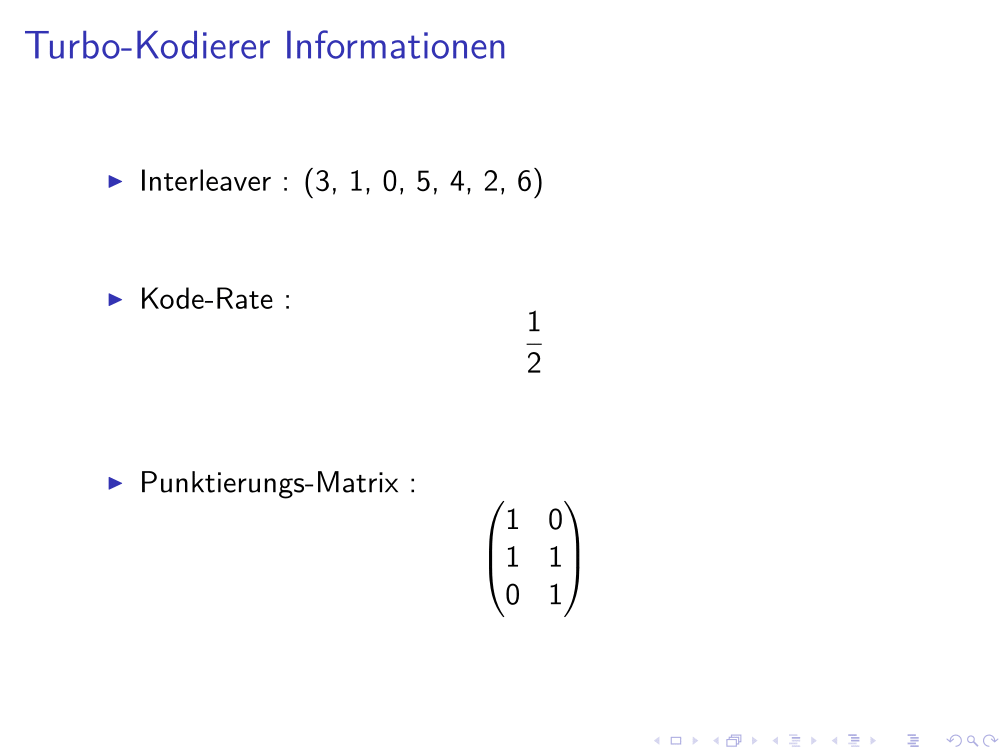
\includegraphics[width=\ScaleIfNeeded]{pictures/TurboEncodePunctured1}
\caption{Turbo-Kodierer Informationen}
\label{pic:TurboCoderInformation}
\end{figure}  

Die genauen Informationen über die Turbo-Kodierer Parameter finden sich auf der Abbildung \ref{pic:TurboCoderInformation}. Dort wird als erstes der Permutationsvektor angezeigt, der beim Interleaver verwendet wird. Das stellt die Reihenfolge der Bits dar, wie sie aus dem Interleaver kommen. Als nächstes wird die Kode-Rate angezeigt, die bei einem normalen Turbo-Kodierer ohne Punktierung immer $\frac{1}{3}$ ist. Hier wird der Wert mit Punktierung berechnet und dargestellt. Am Ende wird noch die Punktierungsmatrix abgebildet.

\begin{figure}[!ht]
\centering
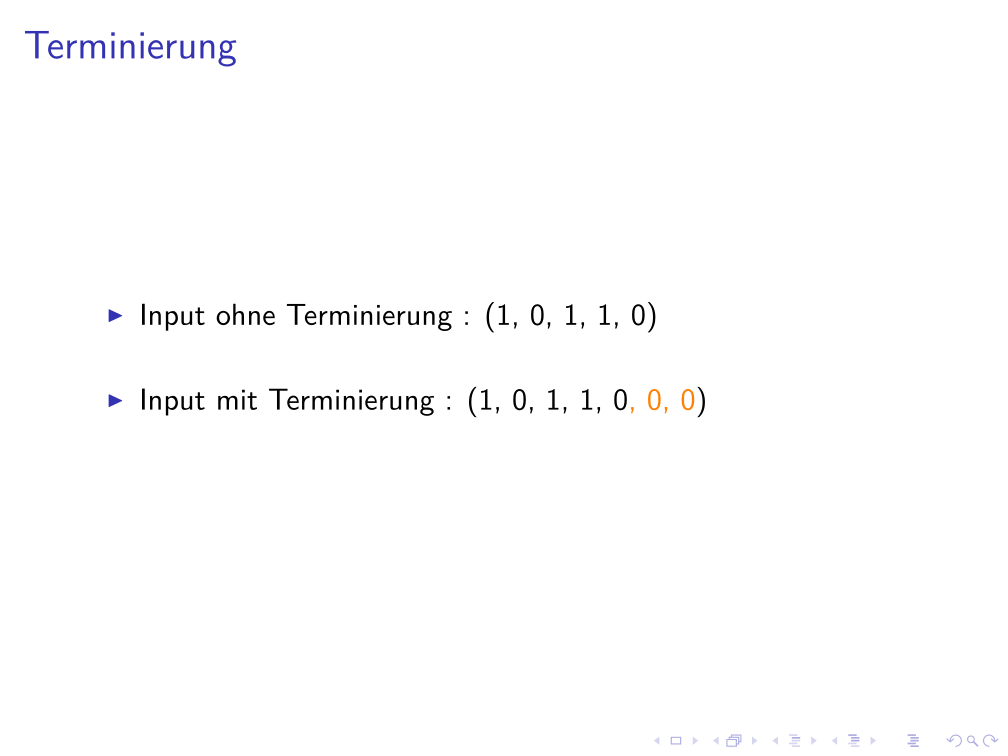
\includegraphics[width=\ScaleIfNeeded]{pictures/TurboEncodePunctured2}
\caption{Terminierung bei der Kodierung}
\label{pic:TerminationEncode}
\end{figure}  

In Abbildung \ref{pic:TerminationEncode} sieht man die Darstellung der Terminierung. Da die Faltungskodierer eine Terminierung vorsehen, muss bei der Eingangsbitfolge noch die Terminierungsbits berechnet werden, damit der Kodierer am Ende im Ausgangszustand ist. Diese Bits werden an die Ausgangsnachricht angefügt und in Orange dargestellt. Bei einem nicht rekursiven Faltungskodierer sind es immer 0er, jedoch bei einem rekursiven müssen sie berechnet werden.

\begin{figure}[!ht]
\centering
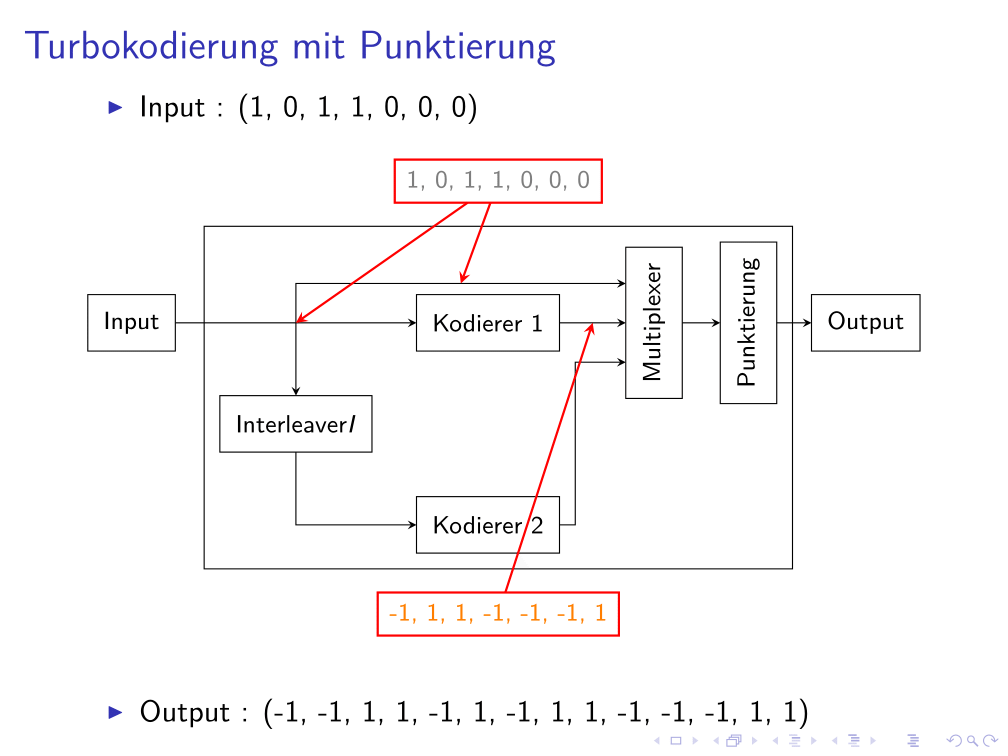
\includegraphics[width=\ScaleIfNeeded]{pictures/TurboEncodePunctured3}
\caption{Turbo-Kode Schaltung}
\label{pic:TurboEncode}
\end{figure}  

Auf der nächsten Folie, die in Abbildung \ref{pic:TurboEncode} dargestellt ist, ist die komplette Schaltung abgebildet, die für die Kodierung nötig ist. Die beiden Kodierer sind die übergebenen Faltungskodierer, die verwendet werden, um einen Teil des resultierenden Signals zu erhalten. Die Bits sind eingefärbt, damit man das Ergebnis nach dem Multiplexer aus den Farben folgern kann. Die drei Einzelbitfolgen werden so ineinander verschachtelt, damit jeweils ein Bit aus Teilfolge eins, zwei und drei hintereinander sind. Das lässt sich am Bestem mit Abbildung \ref{pic:TurboEncodeMultiplexer} zeigen. Dort sieht man sehr leicht, wie der Multiplexer die Bitfolgen ausgibt.

\begin{figure}[!ht]
\centering
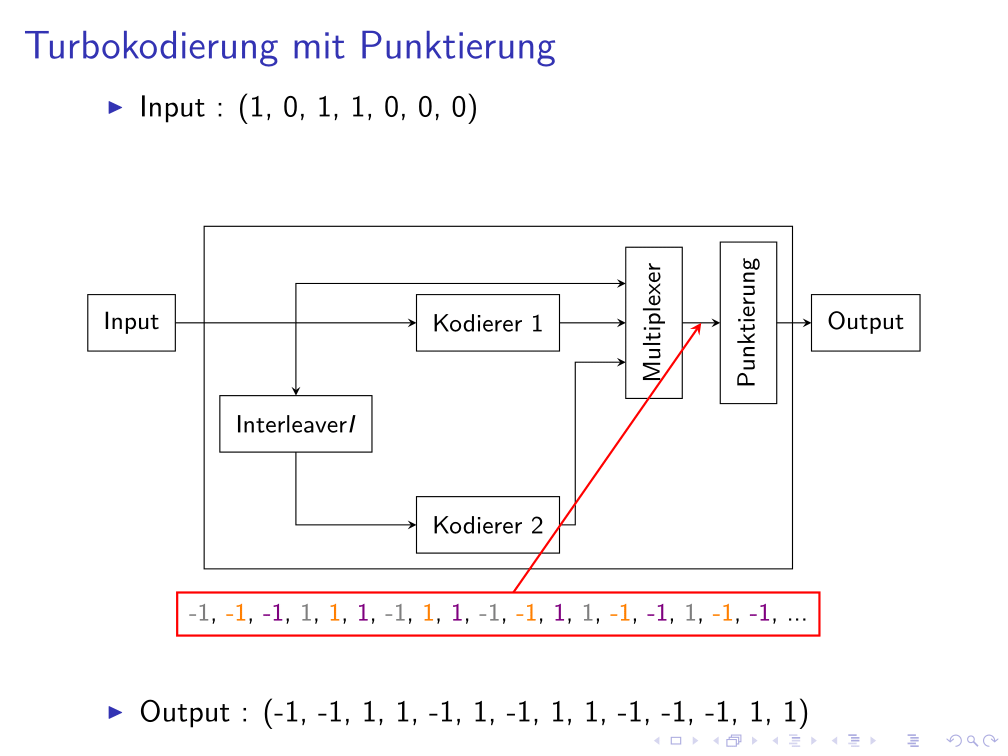
\includegraphics[width=\ScaleIfNeeded]{pictures/TurboEncodePunctured4}
\caption{Multiplexer}
\label{pic:TurboEncodeMultiplexer}
\end{figure}  

\begin{figure}[!ht]
\centering
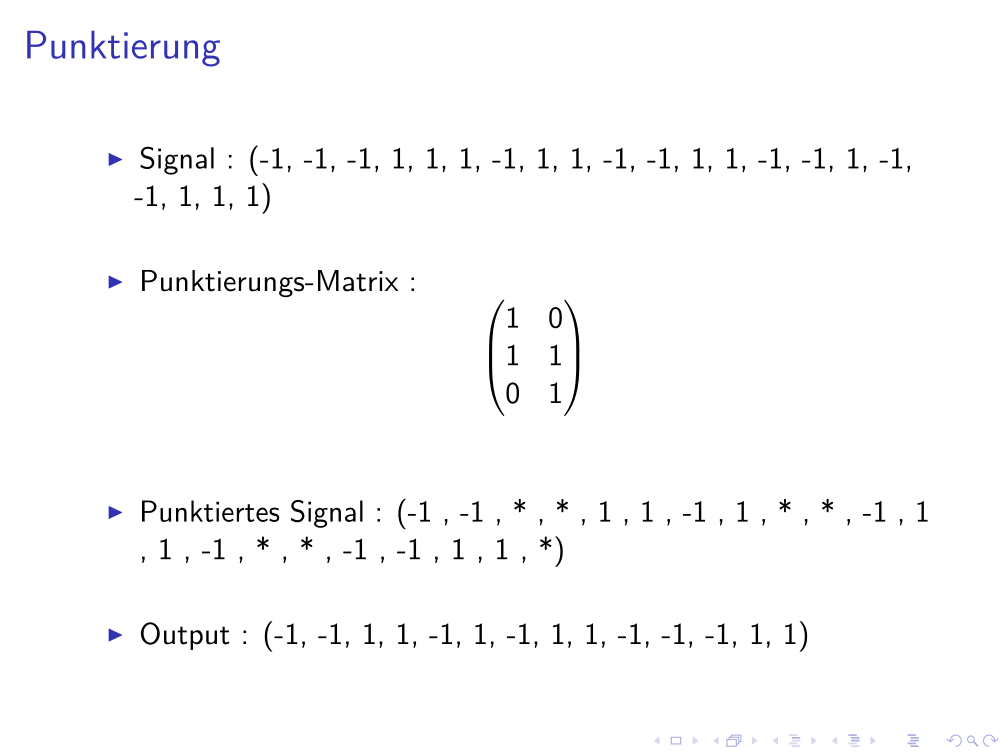
\includegraphics[width=\ScaleIfNeeded]{pictures/TurboEncodePunctured5}
\caption{Multiplexer}
\label{pic:TurboEncodePuncturing}
\end{figure}  

Auf der letzten Abbildung \ref{pic:TurboEncodePuncturing} ist die Punktierung sehr einfach dargestellt. Dabei wird jedes zu löschende Bit mit einem Stern * angezeigt. Somit lässt sich einfach nachvollziehen, dass die Bitfolge von oben nach unten spaltenweise durch die Punktierungsmatrix geführt wird und bei einer 0 dieses Bit entfernt wird. Am Ende ist das fertige Signal dargestellt, das dann auf den Übertragungskanal gelangt. 

Bei der Kodierung ohne Punktierung ist der Ablauf exakt der Selbe, nur wird eben das Signal am Ende nicht punktiert, sondern direkt ausgegeben.

\section{Dekodierung}
\label{sec:visualization_decode}

\section{Simulation}
\label{sec:visualization_simulation}

\subsection{Turbo-Kode}
\label{sec:visualization_simulations_turbo}

\subsection{Kanalkodierung}
\label{sec:visualization_simulations_channelcoding}

\chapter{Beispiele}
\label{cha:examples}
Um dem Benutzer den Einstieg zur Verwendung des Paketes zu erleichtern, sind in den folgenden Kapiteln Beispiele und genaue Erklärungen zu allen wichtigen Funktionen. Dabei wird im Kapitel \ref{sec:example_createHelpers} alle wichtigen Variablen erstellt, die dann in den Kapiteln \ref{sec:example_withPunctuation} und \ref{sec:example_withoutPunctuation} beim Kodieren und Dekodieren verwendet werden. Zum Schluss wird im Kapitel \ref{sec:example_simulations} die verschiedenen Möglichkeiten der Ausführung von Simulationen erläutert.

\section{Erzeugen von Kodierer, Permutationsvektor und Punktierungsmatrix}
\label{sec:example_createHelpers}
Zuerst werden Hilfsvariablen erzeugt, die für die folgende Kodierungs- und Dekodierungsverfahren benötigt werden. Diese Variablen müssen nicht unbedingt mitgegebenen werden, dann werden die Standard-Werte verwendet. Das bedeutet, dass falls keine Punktierungsmatrix übergeben wird, der Standard-Wert \emph{NULL} ist und darum nicht punktiert wird. Ebenfalls wird nicht permutiert, wenn kein Permutationsvektor als Argument übergeben wird. Es wird zwar ein Permutationsvektor benötigt, damit die Interleaver richtig arbeiten können, jedoch wird ein Vektor vom Typ \emph{PRIMITIVE} verwendet, dieser allerdings ändert die Reihenfolge der Bits nicht (root=0). Beim Kodierer verhält es sich ähnlich, jedoch wird hier ein vordefinierter Standard-Faltungskodierer verwendet (\emph{ConvGenerateRscEncoder(2,2,c(5,7))}), dieser wird in allen Turbo-Kode-Funktionen benützt, falls kein eigener Kodierer übergeben wird.

\begin{lstlisting}[caption=Erzeugung von Kodierer und Punktierungsmatrix, label={lst:createHelpersCoderPunctuation}, float=ht]
input <- c(1,0,1,1,0)

coder <- ConvGenerateEncoder(2, 2, c(4,5))

punctuation.matrix <- TurboGetPunctuationMatrix(c(1,1,0))
\end{lstlisting}

Wie im Listing \ref{lst:createHelpersCoderPunctuation} zu sehen ist, wird als allererstes eine zu kodierende Nachricht erzeugt, die dann benötigt wird, die dann benötigt wird um eine Punktierungsmatrix zu bekommen. Anschließend wird ein nicht rekursiver Faltungskodierer, mit der Funktion vom Faltungskode-Teil des Packetes \cite{nocker}, erzeugt. Dabei wurde ein Kodierer mit zwei Registern und zwei Ausgängen gewählt. Wichtig ist, dass der erste Ausgang vom Eingang durchgeschalten wird damit es ein systematischer Kodierer ist. Das wird erreicht, indem das erste Generatorpolynom mit $2^M = 2^2 = 4$ deklariert wird. Zum Schluss wird noch eine Punktierungsmatrix erstellt, die aus nur einer Spalte besteht und jedes dritte Bit aus dem Vektor entfernt. Bei einer 1 wird das Bit behalten, bei einer 0 verworfen.

\begin{lstlisting}[caption=Erzeugung von verschiedenen Permutationsvektoren, label={lst:createHelpersPermutation}, float=ht]
permutation.vector.random <- TurboGetPermutation(length(input), coder, "RANDOM")
permutation.vector.primitve <- TurboGetPermutation(length(input), coder, "PRIMITIVE", list(root=3))

input2 <- c(1,0,1,1,0,1)
permutation.vector.cyclic <- TurboGetPermutation(length(input2), coder, "CYCLIC", list(cols=4, rows=2, distance=2))
permutation.vector.block <- TurboGetPermutation(length(input2), coder, "BLOCK", list(cols=4, rows=2))
permutation.vector.helical <- TurboGetPermutation(length(input2), coder, "HELICAL", list(cols=4, rows=2))
permutation.vector.diagonal <- TurboGetPermutation(length(input2), coder, "DIAGONAL", list(cols=4, rows=2))
\end{lstlisting}

Als nächstes benötigt der Benutzer noch einen Permutationsvektor, dieser wird im Listing \ref{lst:createHelpersPermutation} erzeugt. Dabei wird jeder Typ einmal verwendet. Bei den ersten beiden werden die Eingangsbits von Listing \ref{lst:createHelpersCoderPunctuation} benützt. Da bei den restlichen Typen eine Matrix benötigt wird, muss die Länge der Eingangsbits genau in einer Matrix Platz finden, deshalb wurde ein zweiter Eingangsvektor definiert, der allerdings nur als Demonstration für die anderen Permutationstypen dienen sollte, dieser wird in den weiteren Beispielen nicht weiter verwendet.

\section{Kodieren und Dekodieren ohne Punktierung}
\label{sec:example_withoutPunctuation}
Nachdem alle benötigten Variablen gesetzt wurden kann nun die Kodierung und Dekodierung vorgenommen werden. Dabei wird zuerst ohne Punktierung gearbeitet, jedoch alle anderen zuvor definierten Variablen verwendet.

\begin{lstlisting}[caption=Kodierung und Dekodierung ohne Punktierung, label={lst:encodeDecodeWithoutPunctuation}, float=ht]
encoded <- TurboEncode(input, permutation.vector.random, coder, 2)
encoded
[1] -1 -1 -1  1  1  1 -1  1  1 -1 -1  1  1 -1 -1  1 -1 -1  1  1  1

encoded.noisy <- ApplyNoise(encoded, 0.1)
round(encoded.noisy, 2)
[1] -2.41 -2.36 -0.26  1.06  1.37  0.22  1.13  0.93  0.33 -1.15 -1.18  0.59
[13]  1.32 -0.31 -1.37 -0.01 -1.42 -1.62  2.18  2.29  0.93

decoded <- TurboDecode(encoded.noisy, permutation.vector.random, 5, coder, 2)
decoded
$output.soft
[1]  -1.394185  1.394185  2.775904 -1.394185  2.775904

$output.hard
[1] 1 0 1 1 0
\end{lstlisting}

Der gesamte Vorgang lässt sich in wenigen Zeilen erledigen, wie in Listing \ref{lst:encodeDecodeWithoutPunctuation} zu sehen ist. Zuerst werden einfach die zuvor definierten Variablen der Kodierungsfunktion mitgegeben, als letzter Parameter wird noch der Index des zu verwendeten Ausgangs des Kodierers angegeben (zwei in diesem Fall). Danach erhält man das kodierte Signal mit dem Signalpegel 1 und -1. Dieses Signal wird dann einem Signal/Rausch-Verhältnis von 0.1dB  verrauscht und anschließend ausgegeben, damit man den Unterschied zwischen Originalsignal und Verrauschtem sieht. Dabei werden nur zwei Nachkommastellen ausgegeben, um die Länge der Ausgabe zu kürzen. 

Nachdem das Signal kodiert und übertragen wurde, kann der Empfänger es nun wieder dekodieren. Dabei schickt er das empfangene Signal in die Dekodierungsfunktion, als Iterationsanzahl wird fünf gewählt. Das Ergebnis ist dann eine Liste mit den Soft- und Hard-Werten. Dabei ist zu erkennen, dass positive Soft-Werte auf eine 0 und negative auf eine 1 abgebildet werden. Bei diesem Beispiel ist schön zu sehen, dass auch ein ziemlich verrauschtes Signal vom Turbo-Dekodierer wieder hergestellt werden kann.
\section{Kodieren und Dekodieren mit Punktierung}
\label{sec:example_withPunctuation}

Der gleiche Ablauf kann mit Punktierung wiederholt werden. Dabei wird am Ende des Kodierungsvorgangs die Bits entfernt, bei denen in der Matrix eine 0 steht und die Bits durchgelassen bei denen eine 1 steht. Beim Dekodierungsvorgang wird an den Stellen eine 0 eingefügt, die zuvor entfernt wurden. Da der Signalpegel normalerweise -1 oder 1 ist, wird für die wieder eingefügten Bits eine 0 eingefügt, da unklar ist welche Signalpegel sie tatsächlich haben. Mit einer 0 besteht die gleiche Wahrscheinlichkeit für eine -1 oder 1 an dieser Stelle.

\begin{lstlisting}[caption=Kodierung und Dekodierung mit Punktierung, label={lst:encodeDecodeWithPunctuation}, float=ht]
encoded.punctured <- TurboEncode(input, permutation.vector.random, coder, 2, punctuation.matrix)
encoded.punctured
$original
[1] -1 -1 -1  1  1  1 -1  1  1 -1 -1  1  1 -1 -1  1 -1 -1  1  1  1

$punctured
[1] -1 -1  1  1 -1  1 -1 -1  1 -1  1 -1  1  1

decoded.punctured <- TurboDecode(encoded.punctured$punctured, permutation.vector.random, 5, coder, 2, punctuation.matrix)
decoded.punctured
$output.soft
[1] -6  6 -6 -6  6

$output.hard
[1] 1 0 1 1 0
\end{lstlisting}

Im dargestellten Listing \ref{lst:encodeDecodeWithPunctuation} sieht man nun das Verfahren mit Punktierung. Dort wird als erstes der Kodierfunktion die Punktierungsmatrix mitgegeben. Dadurch werden Bits entfernt, wie man an der Ausgabe sieht. Zurückgeliefert wird eine Liste mit dem Originalvektor ohne Punktierung und einmal der Punktierte, das muss bei der Verwendung dieser Variable bedacht werden. Der Dekodierfunktion wird nun das punktierte Signal mitgegeben und die fügt als erstes die gelöschten Bits wieder ein und dekodiert das Signal dann. Als Resultat bekommt man wieder eine Liste die Soft- und Hard-Werte enthalten. Das Ergebnis nach fünf Iterationen stimmt mit der Ausgangsnachricht überein, somit war die Dekodierung erfolgreich.

\section{Simulationen}
\label{sec:example_simulations}

Die nächsten drei Unterkapitel werden sich den verschiedenen Simulationsfunktionen im Paket beschäftigen. Dabei wird zuerst eine reine Simulation des Turbo-Kode-Verfahrens vorgenommen. Im Anschluss werden alle drei Kanalkodierungsverfahren (Block-, Faltungs und Turbo-Kodes) miteinander verglichen und zum Schluss wird noch die Hilfsfunktion zur Darstellung verschiedener Simulationsergebnisse an einem Beispiel erklärt.

\subsection{Turbo-Kode-Simulation}
\label{sec:example_simulations_turbo}

Im folgenden Beispiel wird eine Simulation des Turbo-Kode-Verfahren durchgeführt, bei der alle Parameter bestimmt werden können, wie Permutationstyp, Länge der Nachricht, Kodierer, zu testende Signal/Rausch-Verhältnisse, Anzahl von Dekodierungsiterationen und Anzahl der Wiederholungen. Als Ergebnis wird ein Dataframe zurückgegeben, das die Bitfehlerrate für jedes Signal/Rausch-Verhältnis beinhaltet.

\begin{lstlisting}[caption=Turbo-Kode-Simulation, label={lst:turboCodeSimulation}, float=ht]
df1 <- TurboSimulation(coder, "DIAGONAL", list(rows=2,cols=501), 3, 1000, 0.01, 0.1, 0.01, 50, punctuation.matrix)
df1
     db     ber
1  0.01 0.11294
2  0.02 0.11430
3  0.03 0.11238
4  0.04 0.11208
5  0.05 0.11050
6  0.06 0.10880
7  0.07 0.10832
8  0.08 0.10784
9  0.09 0.10868
10 0.10 0.10720
\end{lstlisting}

In Listing \ref{lst:turboCodeSimulation} wurde eine Nachrichtenlänge von 1000 Bits gewählt, die zwischen 0.01-0.1dB bei drei Dekodierungsiterationen getestet werden. Nach 50 Durchläufen wird der Mittelwert gebildet und in das zurückgegebene Dataframe geschrieben. Dieses kann entweder im Visualisierungsbericht dargestellt werden (\emph{visualize=TRUE}), oder mit der in Kapitel \ref{sec:example_simulations_plot} vorgestellten Funktion.

\subsection{Kanalkodierungs-Simulation}
\label{sec:example_simulations_channel}

Damit ein Vergleich der drei Kanalkodierungsverfahren möglich ist, müssen alle drei Verfahren mit den gleichen Parameter getestet werden. Danach kann mittels der Bitfehlerrate ein genauer Vergleich angestellt werden und die Vor- und Nachteile der Verfahren analysiert werden.

\begin{lstlisting}[caption=Kanalkodierungs-Simulation, label={lst:channelCodeSimulation}, float=ht]
ChannelcodingSimulation(50, max.db = 1, turbo.decode.iterations = 3)
    db block.ber   conv.ber  turbo.ber
1  0.1 0.1911429 0.05800000 0.06085714
2  0.2 0.1802857 0.06857143 0.05485714
3  0.3 0.2011429 0.06714286 0.05171429
4  0.4 0.1862857 0.06171429 0.03085714
5  0.5 0.1840000 0.04342857 0.03657143
6  0.6 0.1745714 0.06485714 0.03200000
7  0.7 0.1697143 0.05085714 0.03428571
8  0.8 0.1577143 0.03485714 0.02342857
9  0.9 0.1668571 0.04285714 0.02285714
10 1.0 0.1442857 0.03342857 0.01457143
\end{lstlisting}

Bei dem Beispiel in Listing \ref{lst:channelCodeSimulation} wurde eine Nachrichtenlänge von 50 Bits gewählt, die bis maximal 1dB Signal/Rausch-Verhältnis getestet wird und drei Dekodierungsiterationen im Turbo-Dekodierer vorgenommen werden. Bei allen anderen Parameter wurden die Standard-Werte verwendet. Das Ergebnis ist ein Dataframe, das für jedes einzelne Verfahren eine Spalte mit den zugehörigen Bitfehlerraten enthält. Der direkte Vergleich in einer Grafik ist im Visualisierungsbericht enthalten (\emph{visualize=TRUE}). 

\subsection{Vergleich mehrerer Simulationen}
\label{sec:example_simulations_plot}

Nachdem die reinen Dataframes als Rückgabewert der Simulation von Kapitel \ref{sec:example_simulations_turbo} nicht wirklich aussagekräftig sein, ermöglicht die folgende Funktion eine Darstellung verschiedener Simulationen in einer Grafik. Dadurch lassen sich diese miteinander besser vergleiche und genaue Analysen sind möglich.

\begin{lstlisting}[caption=Vergleich mehrerer Simulationen, label={lst:plotSimulations}, float=ht]
df2 <- TurboSimulation(msg.length = 1000, min.db = 0.01, max.db = 0.1, db.interval = 0.01)

PlotSimulationData(df1, df2)
\end{lstlisting}

\begin{figure}[ht]
\centering
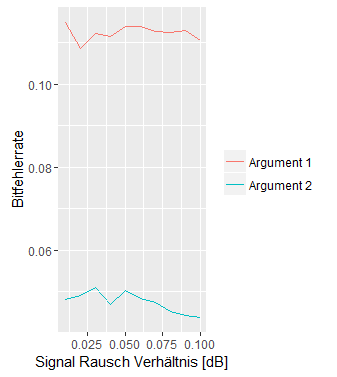
\includegraphics[width=\ScaleIfNeeded]{pictures/PlotSimulations}
\caption{Vergleich zweier Simulationen}
\label{pic:plotSimulations}
\end{figure}

Im Listing \ref{lst:plotSimulations} werden zwei verschiedene Simulationen mit unterschiedlichen Kodierern miteinander verglichen. Die erste Simulation stammt noch von Kapitel \ref{sec:example_simulations_turbo}, diese wird mit der Simulation des Standard-Kodierers verglichen. Die erstellte Grafik ist in Abbildung \ref{pic:plotSimulations} zu sehen, da ist deutlich zu erkennen, dass die erste Simulation klar die besseren Ergebnisse liefert.

\chapter{Fazit, Ausblick, Erweiterungen}
\label{cha:result}
Das Ziel der Bachelorarbeit war die Erstellung eines R-Paketes zur Umsetzung des  Turbo-Kode-Verfahrens, welches eine Kanalkodierung darstellt. Dabei stand im Mittelpunkt der didaktische Nutzen für zukünftige Studierende. Deswegen bietet das Paket lehrreiche Visualisierungen der Kodierung und Dekodierung an. Dadurch soll das Verständnis der Verfahren erleichtert werden. Noch dazu werden Berichte bei den Simulationen erstellt, die eine einfache Analyse der Leistungsfähigkeit der verschiedenen Kanalkodierungsverfahren zulässt.

Die beiden alternativen Verfahren, Blockkodes und Faltungskodes, wurden von den Kollegen Nocker \cite{nocker} und Wimmer \cite{wimmer} in ihren Bachelorarbeiten umgesetzt. Alle drei Kodierungen wurden in ein gemeinsames Paket verpackt. Somit ist ein kompaktes R-Paket entstanden, das alle Kanalkodierungsverfahren beherrscht und dadurch vielseitig einsetzbar ist.  

Als Erweiterung der vorhandenen Funktionalität würde sich eine Ausweitung der Visualisierungen auf längere Nachrichten anbieten. Dadurch könnte die Darstellung auf mehr als 18 Bits erweitert werden. Das Turbo-Kode-Verfahren könnte auf die Verwendung von Blockkodes ausgeweitet werden. Zusätzlich zur parallelen wäre die iterative Verkettung interessant, da dies die ersten Ansätze von der Kodeverkettung waren. Als alternativer Algorithmus bei der Dekodierung könnte der aufwändigere BCJR-Algorithmus implementiert werden, der bei längeren Nachrichten leistungsfähiger als der Viterbi-Algorithmus ist \cite[233-236]{schoenfeld2012informations}.

\cleardoublepage%

\listofabbreviations
\clearpage

\listoffigures
\clearpage

\listoftables
\clearpage

\lstlistoflistings
\clearpage

\printbibliography
\end{document}